\documentclass[11pt]{article}

\usepackage[a4paper,left=0.5in,right=0.5in,top=0.4in,bottom=0.4in,%
            footskip=.25in]{geometry}
\usepackage{graphicx}
\usepackage{gensymb}
\usepackage{amsmath}
\usepackage{siunitx}
\usepackage[nottoc]{tocbibind}
\usepackage[titletoc]{appendix}
\usepackage{titlesec}
\usepackage{caption}
\usepackage{listings}
\usepackage{amsfonts}
\usepackage[list=true,listformat=simple]{subcaption}
\usepackage{amsmath}
\usepackage{float}
\usepackage{url}
\usepackage{placeins}
\usepackage{natbib}

\usepackage{subcaption}

\setcounter{secnumdepth}{4}

\usepackage{color} %red, green, blue, yellow, cyan, magenta, black, white
\definecolor{mygreen}{RGB}{28,172,0} % color values Red, Green, Blue
\definecolor{mylilas}{RGB}{170,55,241}

\usepackage{hyperref}
\hypersetup{
  pdftitle={assignment-540XXXXXX},
  pdfauthor={51044041},
  colorlinks = true,
  linkcolor = black,
  anchorcolor = black,
  citecolor = black,
  urlcolor = blue
}
\usepackage{color, colortbl}
\usepackage[first=0,last=9]{lcg}
\definecolor{LightCyan}{rgb}{0.88,1,1}
\definecolor{ForestGreen}{rgb}{0.24,1,0.24}
\usepackage[table]{xcolor}
\usepackage{tikz}
\usetikzlibrary{matrix,calc}

\lstset{language=Matlab,%
            basicstyle=\tiny,
            %basicstyle=\color{red},
            breaklines=true,%
            morekeywords={matlab2tikz},
            keywordstyle=\color{blue},%
            morekeywords=[2]{1}, keywordstyle=[2]{\color{black}},
            identifierstyle=\color{black},%
            stringstyle=\color{mylilas},
            commentstyle=\color{mygreen},%
            showstringspaces=false,%without this there will be a symbol in the places where there is a space
            numbers=left,%
            numberstyle={\tiny \color{black}},% size of the numbers
            numbersep=9pt, % this defines how far the numbers are from the text
            %emph=[1]{for,end,break},emphstyle=[1]\color{red}, %some words to emphasise
            %emph=[2]{word1,word2}, emphstyle=[2]{style},    
}

\begin{document}

    \thispagestyle{empty}
    
    \begin{center}
        \vspace*{30mm}

            \textsc{The University of Sydney}\\
        \vspace{5mm}
            \textsc{Project Report Submission}\\
        \vspace{20mm}

        \hrule
        \vspace{8mm}
            \begin{LARGE}
                \textbf{Final Report: Machine Algorithms to Predict Machine Failure}
            \end{LARGE}\\
        \vspace{8mm}
        \hrule

\vspace{20mm}
\begin{table}[h]
    \centering
    \begin{tabular}{|l|l|l|}
        \hline
        \textbf{Name} & \textbf{Student ID} & \textbf{Contribution} \\ \hline
        Yarra Al-hattab & 540657704 & \\ \hline
        Loklan Duong & 510440471 &  \\ \hline
        Thomas Ishak & 540756443 &  \\ \hline
        Kenton Lee & 540745333 & \\ \hline
    \end{tabular}
\end{table}

        \vspace{15mm}
\begin{center}
    \begin{minipage}{0.5\linewidth}
        \centering
        \textit{A report submitted in partial fulfillment for 
        the Unit of Study ENGG2112: Multi-disciplinary Engineering}
    \end{minipage}
\end{center}
        \vspace{16mm}

        
\includegraphics[width=30mm]{figures/USYD_logo.png}\\
        \vspace{3mm}
        \begin{text}
            School of AMME\\
            \vspace{2mm}
            University of Sydney\\
            \vspace{2mm}
            Australia\\
            \vspace{10mm}
            September, 2025\\
        \end{text}
    \end{center}


    \pagebreak
    
\pagenumbering{roman}

\section*{Abstract}

In industrial environments, equipment failures often lead to very costly downtimes, safety hazards, and reduced operational efficiency. Reliance on only scheduled maintenance and reactionary protocols limits efficiency and fails to address the issues across different machine types. This report will investigate these issues and, in turn, propose a predictive maintenance machine learning algorithm that aims to improve reliability and safety.\\

Three datasets were analysed to train, evaluate, and optimise supervised learning models - Logistic Regression, K-nearest neighbours, Random Forest, and Gradient Boosted Trees. Each dataset represented different industrial environments and data characteristics that ranged from environmental sensors to mechanical stress indicators. Data preprocessing steps were implemented of which included outlier removal, feature scaling, and class balancing to improve data consistency and reduce any model bias.\\

Across all three datasets, Random Forest and Gradient Boosting Trees were proven to be the most effective and accurate, reaching over 95\% accuracy when placed in complex environments. These ensemble models were chosen as they are best suited for diverse industrial datasets due to their stability and interpretability. Feature importance and SHAP analysis revealed that the strongest contenders in predicting machine failure were mechanical and environmental variables such as torque, tool wear, and vibration frequency. \\

Overall, this study confirms that predictive maintenance systems that are powered by ML models can substantially enhance operational safety and reliability and increase cost efficiency. The proposed integrated app will allow users to gather real-time data ready for continuous monitoring and fault prediction. Future development will focus on expanding our dataset diversity and effectively introducing multiclass fault classification. 




\newpage
\tableofcontents
\newpage

\pagenumbering{arabic}


\section {Background and Motivation}
%%  Provides a thorough, well-supported, and logically connected overview of the background, precisely describing the data characteristics, sourcing, and relevance. States the problem clearly, concisely, and consistently aligned with the background. Objectives are highly relevant, directly linked to the work performed, demonstrate insightful understanding of the problem, and thoughtfully identify potential beneficiaries or broader impacts.

Reliable operation of heavy machinery is essential to numerous industries, from manufacturing to transportation and infrastructure, where failure of equipment can result in potential injuries, fatalities, and significant financial losses. The current approach to machine maintenance follows a manual inspection-based approach, heavily prone to retraining issues and human error, which magnifies the consuming, risky, and unreliable nature of the current practice. A shift to predictive - rather than reactive - maintenance approaches is being adopted in Australian industry, as reflected in asset management standards such as AS ISO 55001:2024. Our concept aims to augment upon this and propel forward a safe and reliable industrial world.\\

Machine learning enabled predictive maintenance provides a solution to these issues, supporting studies which have shown that implementing these systems on machinery can reduce maintenance costs by 25\% to 30\% \cite{Fernandes2022}. Data-driven maintenance can also improve operational safety and prolong the equipment's overall lifespan. This also leads to an increase in production efficiency as it reduces unexpected downtime and improves resource allocation \cite{Lei2020}, where 146,700 serious workplace injury claims are made to Safework Australia annually, with equipment failures representing a significant preventable cause \cite{safeworkaustralia2025}. The outcomes of this project will help manufacturing factories, maintenance engineers, and industrial operators by lowering operating costs and downtime while still ensuring workers' safety. More broadly, implementing this ML can reduce material waste, maximise energy consumption, and minimise dangerous mechanical failures that could put employees or the local community at risk. The effective application of this predictive maintenance can then help promote sustainable industrial growth. So, the shift from manual to intelligent maintenance could have major positive effects on society, the economy, and technology.



\section {Objectives and Problem Statement}

%%  Provides a thorough, well-supported, and logically connected overview of the background, precisely describing the data characteristics, sourcing, and relevance. States the problem clearly, concisely, and consistently aligned with the background. Objectives are highly relevant, directly linked to the work performed, demonstrate insightful understanding of the problem, and thoughtfully identify potential beneficiaries or broader impacts.

\subsection{Problem Statement}

Despite the major advances in automation and data collection, the Australian industrial field still lacks precise and broadly applicable predictive systems that can anticipate machine failure far before its occurrence. Any pre-existing systems are tailored to their specific machine details and require extensive background knowledge to both understand and then implement the system from the given data. This limits the widespread application of machine learning as an easily adoptable approach towards safety. In frequently used industrial settings, failure to proactively identify malfunctions results in expensive downtime, higher maintenance costs, and safety hazards. This project aims to address and fix this gap by developing and comparing supervised learning models that are trained on various arrays of environmental and sensor datasets to predict machine failure. The ultimate objective is to develop a strong, data-driven predictive maintenance framework that increases workplace safety, lowers financial losses, and improves reliability across industrial sectors. This study uses international datasets as a proof-of-concept to demonstrate the viability of supervised learning approaches, with the understanding that deployment in Australian industry would require validation on local equipment and operating conditions.

\subsection{Our Approach}

Our approach reflects on the various arrays of collected data from the industrial field, which has such a broad scope of machinery; however, it still provides a streamlined and widely adoptable pathway to implementing machine learning to increase safety and boost productivity. By performing our analysis on three separate datasets with varying input features, we can tailor our findings to a combination of circumstances that users, such as plant operators, machine drivers, or mechanical maintenance crews, may experience. This recommends them an optimised model for their supplied input features to then provide foresight into their machine failure.

\section{Methodology}

%%  Provides a clear, systematic, and logically sequenced explanation of methods, explicitly detailing the ML algorithm conception and design, supported with appropriate mathematics, pseudo-code, and real-world examples. Thorough justification of parameter and hyperparameter choices, including a critical discussion of trade-offs specific to ML model design and optimisation.

\begin{figure}[H]
    \centering
    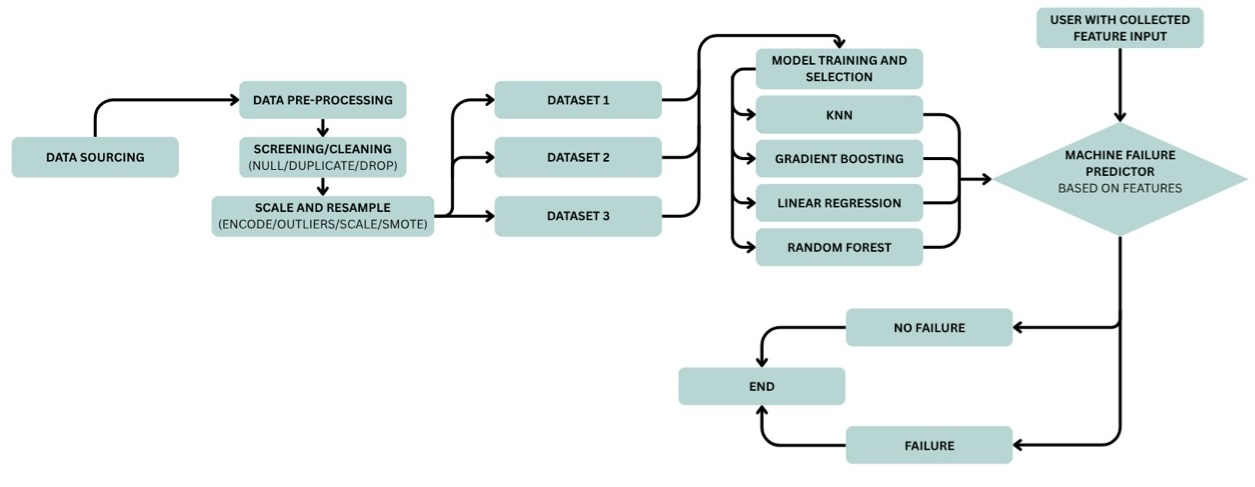
\includegraphics[width=1.05\textwidth]{figures/Industrial machine failure.jpg} 
    \caption{Methodology Flowchart}
    \label{fig:method}
\end{figure}
\subsection{Data Collection}
\subsubsection{Dataset 1}
The first dataset – sourced from Kaggle \cite{kaggle2023a} – consists of 944 observations and includes 10 features: footfall, tempMode, AQ, USS, CS, VOC, RP, IP, and Temperature. Our target column being Fail. This dataset presents an industrial context where these environmental variables can be used to predict machine failure. It is a well-suited dataset as it is moderately sized and has features that can often be seen in places of industrial work, as well as being well-suited for training and evaluation of classification models. The class distribution shows 551 No-Failure samples (58.4\%) and 393 Failure samples (41.6\%), resulting in an imbalance ratio of approximately 1.4:1. This indicates that the dataset is only slightly imbalanced, meaning both classes are relatively well represented and suitable for balanced model training without extensive resampling.

\subsubsection*{Distributions and Correlations}
From the histograms in Figure \ref{fig:histograms_dataset1}, we can observe a mix of distribution types across the different features. Variables such as footfall, USS, and CS show very highly skewed distributions, with most values being near zero and then followed by a long tail of higher values. This is typical of data that is based on counters or the amount of use, where high readings are rare but significant when they do occur. Other variables, such as AQ and Temperature, show more symmetrical distributions, which could indicate some sort of sensor grouping or specific re-occurring operational states. Finally, variables such as tempMode and IP are discretised, showing more categorical histograms. RP is almost normally distributed with a slight left skew, this suggests a much more balanced range of values.

\subsubsection*{Outlier and Spread Analysis}
The boxplots shown in Figure \ref{fig:boxplot_dataset1} further highlight the variability from this dataset and prove the presence of many outliers. Footfall, USS, and Temperature contain a significant number of outliers. This is unlikely to be a data error and is probably real operational anomalies; however, they may negatively affect the model performance, specifically ones that operate based on variance and scale, such as KNN. The rest of the features have more compacted IQRs with less extreme values, which can suggest more consistent behaviour.\\\

Overall, this dataset provides a strong foundation for applying and testing ML models for predictive maintenance. The mix of skewed and balanced distributions and observable outliers reflects real-world outcomes, which will make our model more realistic and reliable.

\subsubsection{Dataset 2}
The second dataset – also sourced from Kaggle \cite{kaggle2023b} – contains 10,000 observations capturing sensor data from industrial machinery. We will be using 6 main features: Air temperature, Process temperature, Rotational speed, Torque, Tool wear, and Type\_Encoded. The target column is failure type. It is well-suited as it contains a very high volume of data points, which can help us reduce variance in training our models, as well as containing features that are indicative of operating conditions and mechanical stress, which will need to be monitored for predictive maintenance tasks. This dataset will be used to teach our ML models how to predict equipment failure and to detect any abnormal behaviour based on real-time sensor data. The dataset is multi-class, containing several distinct failure types; however, the fault-type classification will not be used due to severe class imbalance. The class distribution shows 9652 No-Failure samples (96.5\%), 112 Heat Dissipation Failure samples (1.1\%), 95 Power Failure samples (0.9\%), 78 Overstrain Failure samples (0.8\%), 45 Tool Wear Failure samples (0.4\%), and 18 Random Failure samples (0.2\%), resulting in an imbalance ratio of approximately 27:1 when comparing no failure to the sum of failure samples.

Binary classification is being used for Dataset 2 because even with techniques like SMOTE, the extreme imbalance across multiple rare fault types, (some individual ratios are exceeding 500:1) would cause the model to overfit synthetic minority samples and fail to generalise.

\subsubsection*{Distributions and Correlations}
Examining the histograms from the figure \ref{fig:histograms_dataset2}, we can see that features such as Air temperature and Torque display a relatively symmetrical and multimodal distribution, which suggests a mix of operating conditions. Rotational speed and Process temperature show mild skewness, with Torque being far right-skewed. This may indicate that most operations occur at lower speeds and have very few high-speed outliers. Tool wear seems to be increasing steadily and then peaks, which is consistent with the usage cycles of most tools. Finally, Type\_Encoded shows some class imbalance as one machine type heavily dominates any other in the dataset.

\subsubsection*{Outlier and Spread Analysis}
Observing the boxplots from fig \ref{fig:boxplot_dataset2} further shows the spread of each variable. Air temperature, Torque, and Tool wear show a mostly contained IQR with a few extreme outliers. On the other hand, Process temperature and Rotational speed display a much larger amount of very extreme outliers. This might correspond to highly specific and rare operating conditions. These outliers may skew some models, but they do offer valuable information about stress thresholds that could explain how and when tool wear occurs, which can help our ML model predict machine failure.\\\

Overall, Dataset 2 offers highly applicable information for our predictive maintenance analysis. The combination of the large amount of data, as well as realistic features and a reasonable class imbalance, ensures that the models we train on this data will have strong relevance in industrial settings. The large number of outliers and skewed distributions will require some preprocessing, but it also reflects the reality of industrial machine operations under varied load conditions. 

\subsubsection{Dataset 3}

The third dataset used in this project is an industrial fault detection dataset comprising sensor readings from an industrial system sourced from kaggle \cite{kaggle2023c} and has 1000 observations. It contains 9 usable features: Temperature, Vibration, Pressure, Flow Rate, Current, Voltage, and the first frequency components from the FFT transformation of Temperature, Vibration, and Pressure, respectively. The target column is Fault. This dataset is generated to simulate fault conditions in a controlled industrial environment and is commonly used in machine learning applications for anomaly and fault detection. It is well-suited for this project as it allows testing of model strength in identifying abnormal system behaviour, where real-world fault data is often limited. The dataset includes four classes representing different operational conditions. The class distribution shows 725 Normal Operation samples (72.5\%), 95 Overheating Fault samples (9.5\%), 91 Leakage Fault samples (9.1\%), and 89 Power Fluctuation Fault samples (8.9\%), resulting in an imbalance ratio of approximately 8.15:1.

\subsubsection*{Distributions and Correlations}

From the histograms in fig \ref{fig:histograms_dataset3}, we can observe that most features follow a normal distribution centred around 0. This suggests that the dataset has been standardised, making it compatible with models that assume normally distributed data, such as Logistic Regression. Variables such as Temperature, Pressure, and Vibration display symmetrical shapes, indicating balanced readings across operating ranges. Meanwhile, features derived from FFT components show slightly wider spreads, likely representing variations in frequency responses caused by potential fault signals. This mix of time-domain and frequency-domain features provides a comprehensive representation of both steady-state and transient system behaviour.

\subsubsection*{Outlier and Spread Analysis}

The boxplots shown in fig. \ref{fig:boxplot_dataset3} highlights that most variables have compact interquartile ranges with relatively symmetrical distributions around their medians. However, outliers are present in almost every feature, most notably in Flow Rate, Voltage, and the FFT-transformed variables. These outliers could indicate fault problems rather than noise, which makes them very useful for model learning. Although little, they could affect the performance of certain models that are more sensitive to extreme values than others, such as KNN or Linear Regression. On the other hand, including them may enhance the model’s ability to detect rare but critical operational anomalies.\\\

Overall, Dataset 3 provides a strong foundation for evaluating fault detection algorithms. The combination of time and frequency domain features ensures that the model can capture different types of industrial abnormalities. Its distributions are standardised and have a realistic spread, which makes the dataset highly applicable for machine learning that are aimed at identifying early signs of system faults in industrial industries.


\subsection{Data Pre-processing}

To enhance our data quality and ensure consistency across all three datasets, a preprocessing pipeline was applied before we began model training. Each dataset underwent the following stages: null value removal, duplicates removal, categorical encoding, feature scaling, outlier detection and removal, and class balancing. These steps will ensure our data will provide the clearest and accurate model and prevent any bias that may occur during evaluation.\\

The outlier detection and removal method was conducted by using the IQR method. This method calculates the first and third quartiles for each feature and checks which of them are in 'acceptable' data boundaries. These boundaries were defined as values that are within 1.5*IQR of these quartiles. Any and all data points that fell outside of this range were then flagged and consequently removed from the dataset. This allowed us to remove extreme sensor readings but still allowed us to keep realistic operational data as although some may appear to be extremely high, it is still something that could occur.\\

All continuous variables were standardized using StandardScaler to transform features to zero mean and unit variance. This prevents features with large numerical ranges from disproportionately influencing distance-based algorithms such as KNN and ensures consistent model comparison across all algorithms. The Synthetic Minority Over-sampling Technique (SMOTE) was applied to balance target classes by generating synthetic minority samples through interpolation between existing  samples and their nearest neighbors. SMOTE was applied only to the training set after the train-test split, otherwise it would cause data leakage and invalidate the testing data. SMOTE generates synthetic samples that may not represent 
physically realisable machine states, potentially causing the model to learn 
unrealistic failure patterns. This risk is mitigated through cross validation and testing on real holdout data. Despite this limitation, SMOTE was chosen for its effectiveness in addressing the severe class imbalance in some of the datasets.

\subsubsection{Model Selections}

The models we chose that best aligned with the project's objectives were Logistic Regression, Random Forest, Gradient Boosted Trees, and K-Nearest Neighbours. These were selected to balance interpretability, robustness, and adaptability to the many different industrial data types. Logistic Regression provides a baseline that is suitable due to its interpretability and much lower computational cost. It is easy to understand and allows for a direct grasp of how each feature contributes to machine failure likelihood. KNN was selected as it's little training assumptions make it suitable for environments that do not have linear patterns, and it works well with smaller datasets, such as one of the ones that we had sourced. It also shows a good evaluation of how well local similarity measures perform when it comes to failure prediction. Random Forest offers robustness to noise and overfitting, which we will come to learn was one of our biggest issues that we had to face. This type of data is very common when it comes to industrial sensor data, and Random Forest also easily helps us identify the most critical values that affect machine failure. Finally, Gradient Boosted Trees was chosen to test the utmost bound of model accuracy and adaptability. Once again, its ability to handle complex and non-linear relationships is extremely useful in this context and should, in theory, achieve better accuracy and reduce bias. Support Vector Machines and Neural Networks were excluded. SVMs become computationally expensive for datasets of 10,000+ samples, and Neural Networks typically require larger datasets than available here to avoid overfitting.



\subsubsection{Dataset 1}
The first dataset had no missing values but had many duplicate entries, which were removed. Categorical values - TempMode and Fail - were label encoded, and continuous features - footfall, AQ, USS, CS, VOC, RP, IP, and Temperature - were scaled using StandardScaler. Any and all outliers were detected and removed to reduce skew, and class imbalance was addressed through SMOTE.

\begin{table}[h!]
\centering
\begin{tabular}{l c c c c c}
\hline
\textbf{Model} & \textbf{Accuracy} & \textbf{Precision} & \textbf{Recall} & \textbf{F1 Score} & \textbf{ROC AUC} \\ 
\hline
KNN                 & 0.875912 & 0.863636 & 0.876923 & 0.870229 & 0.933226 \\
Logistic Regression & 0.883212 & 0.876923 & 0.876923 & 0.876923 & 0.942521 \\
Random Forest       & 0.883212 & 0.888889 & 0.861538 & 0.875000 & 0.952030 \\
Gradient Boosting   & 0.883212 & 0.901639 & 0.846154 & 0.873016 & 0.950214 \\

\hline
\end{tabular}
\caption{Performance Metrics for Dataset 1}
\label{tab:model_performance1}
\end{table}

The Random Forest model achieved the strongest performance of the four for dataset 1 and so will be chosen for further tuning. Figure \ref{fig:all_models_dataset1} shows all models stacked.

\subsubsection{Dataset 2}
The second dataset's null and duplicate values were all removed. Categorical features - Type and Failure Type - were label encoded to numeric form (Type\_Encoded and Failure\_Type\_Encoded). Some features that did not provide adequate information were dropped - UDI, Product ID, Target, Type, and Failure Type. Continuous variables - Type\_Encoded, Air Temperature, Process Temperature, Rotational Speed, Torque, and Toolwear - were scaled using StandardScaler. Outliers were removed, and SMOTE was applied to correct class imbalance.


\begin{table}[h!]
\centering
\begin{tabular}{l c c c c c}
\hline
\textbf{Model} & \textbf{Accuracy} & \textbf{Precision} & \textbf{Recall} & \textbf{F1 Score} & \textbf{ROC AUC} \\ 
\hline
Logistic Regression & 0.797800 & 0.104513 & 0.830189 & 0.185654 & 0.889802 \\
Random Forest       & 0.959665 & 0.390909 & 0.811321 & 0.527607 & 0.946888 \\
Gradient Boosting   & 0.981142 & 0.630769 & 0.773585 & 0.694915 & 0.955168 \\
KNN                 & 0.905186 & 0.198113 & 0.792453 & 0.316981 & 0.904451 \\
\hline
\end{tabular}
\caption{Performance Metrics for Dataset 2}
\label{tab:model_performance2}
\end{table}

The Gradient Boosted model achieved the strongest performance of the four for dataset 2 and so will be chosen for further tuning. See fig.\ref{fig:all_models_dataset2}.

\subsubsection{Dataset 3}

The third dataset was already standardised, so it contained no missing or duplicate values and no encoding was required. Outliers across sensor and FFT-transformed variables, however, were removed to handle unrealistic readings. The remaining features were scaled for consistency, and SMOTE was applied as many faulty types were very underrepresented.


\begin{table}[h!]
\centering
\begin{tabular}{l c c c c c}
\hline
\textbf{Model} & \textbf{Accuracy} & \textbf{Precision} & \textbf{Recall} & \textbf{F1 Score} & \textbf{ROC AUC} \\ 
\hline
Logistic Regression & 0.2903 & 0.6042 & 0.2903 & 0.3603 & 0.5688 \\
Random Forest       & 0.6065 & 0.5231 & 0.6065 & 0.5617 & 0.7908 \\
Gradient Boosting   & 0.6194 & 0.5509 & 0.6194 & 0.5819 & 0.7954 \\
KNN                 & 0.4000 & 0.5520 & 0.4000 & 0.4539 & 0.6537 \\
\hline
\end{tabular}
\caption{Performance Metrics for Dataset 3}
\label{tab:model_performance3}
\end{table}


The Gradient Boosted model achieved the strongest performance of the four for dataset 3 and so will be chosen for further tuning. For this multi-class dataset, the AUC is calculated using micro averaging, where all true positive and false positive rates are aggregated. The AUC is then based on this total count. See fig.\ref{fig:all_models_dataset3}.

\subsection{Training}

\subsubsection{Dataset 1}
For Dataset 1, the Random Forest model was chosen because of its superior performance in overall metrics, specifically recall, as predicting true failures is a critical objective.

The baseline model was trained using a train-test split with a test size of 20\% and then trained on the train split and tested amongst the test split, and performance metrics were produced.  

For the refined model, hyperparameter tuning was completed by using Randomised Search Cross-Validation. This approach searches within a specified range using random combinations to determine the best hyperparameters. To reduce overfitting, the search space was refined by limiting max\_depth, increasing min\_samples\_split and min\_samples\_leaf, which had a great influence on whether or not the model was overfitting. The best hyperparameters found from the Randomised Search Cross-Validation were:

\begin{itemize}
    \item \textbf{n\_estimators}: 150
    \item \textbf{min\_samples\_split}: 5
    \item \textbf{min\_samples\_leaf}: 20
    \item \textbf{max\_features}: \texttt{'sqrt'}
    \item \textbf{max\_depth}: 5
    \item \textbf{criterion}: \texttt{'gini'}
\end{itemize}

The Cross-Validation Recall was 0.9480, which showed that the model was able to generalise pretty well across different folds when searching for the best hyperparameters. The results between the baseline and tuned models can be seen below:

\begin{table}[h!]
\centering
\begin{tabular}{l c c c c c}
\hline
\textbf{Model Version} & \textbf{Accuracy} & \textbf{Precision} & \textbf{Recall} & \textbf{F1 Score} & \textbf{ROC AUC} \\ 
\hline
Baseline Model & 0.8832 & 0.8889 & 0.8615 & 0.87500 & 0.9520 \\
Tuned Model    & 0.8832 & 0.8769 & 0.8769 & 0.87690 & 0.9536 \\
\hline
\end{tabular}
\caption{Performance of the Random Forest model before and after tuning on Dataset 1.}
\label{tab:rf_tuning_dataset1}
\end{table}

Comparing the two models, we observe that the tuned model generalises better than the baseline with a slight increase in Recall, F1 Score and ROC. The ROC curve comparison supports this and shows a slight improvement when comparing them as seen in fig.\ref{fig:roc_dataset1}. The model achieves 87.7\% recall, meaning it misses approximately 12\% of failures. In safety-critical applications, this failure detection rate must be evaluated against the cost and consequences of missed failures.

\subsubsection{Dataset 2}

The Gradient Boosted tree model was selected for Dataset 2 because it performed the strongest out of all the models. To improve its generalisation, the model was trained with a 10\% validation fraction for early stopping, meaning that it stopped if no improvement was observed for 10 iterations, with a tolerance of 0.0001. This setup helps prevent the model from capturing relevant patterns whilst not overtraining on the dataset.

Hyperparameter tuning was performed using Randomised Search Cross-Validation. To reduce overfitting, the search considered lower learning rates, shallower trees, higher minimum samples for splits and leaves, subsampling for both rows and features, and controlled numbers of estimators.

The best hyperparameter configuration identified through this process was: learning\_rate 0.1, max\_depth 5, max\_features 'sqrt', min\_samples\_leaf 7, min\_samples\_split 12, n\_estimators 134, and subsample 0.7. The best cross-validation F1 score was 0.9800, indicating that the model performed consistently across folds during tuning.

\begin{table}[h!]
\centering
\begin{tabular}{l c c c c c}
\hline
\textbf{Model Version} & \textbf{Accuracy} & \textbf{Precision} & \textbf{Recall} & \textbf{F1 Score} & \textbf{ROC AUC} \\ 
\hline
Baseline Model & 0.9300 & 0.3500 & 0.8400 & 0.4800 & 0.9600 \\
Tuned Model    & 0.9586 & 0.3860 & 0.8302 & 0.5269 & 0.9537 \\
\hline
\end{tabular}
\caption{Performance of the Gradient Boosted Tree before and after tuning on Dataset 2.}
\label{tab:gbt_tuning_dataset2}
\end{table}

ROC curve comparison can be seen in \ref{fig:all_models_dataset2}. Compared to the baseline, the tuned model shows a more balanced trade-off between precision and recall while maintaining strong overall discriminative ability. The model achieves 83\% recall with 38.6\% precision after tuning. This reflects the severe class imbalance in the original data (27:1). This means the model correctly identifies 83\% of failures but produces false alarms 61.4\% of the time. 

This precision-recall trade-off reflects the severe class imbalance and the decision to prioritize catching failures (high recall) over minimizing false alarms (low precision), a reasonable choice for safety-critical applications where missed failures are more costly than false alarms, but one that requires operational acceptance of frequent false positives.


\subsubsection{Dataset 3}

The Gradient Boosted Tree was the best model for dataset 3, however, the baseline model was already relatively weak. After tuning, the training accuracy increased to 84\%, but the test accuracy dropped sharply to 39\%, which is a clear indication of overfitting. The lower AUC of 0.68 further confirms that the model struggles to generalize to unseen data. To address this, the model was further refined using more conservative hyperparameters and a slightly larger validation fraction. The model was trained with a 15\% validation set for early stopping, halting if no improvement over 10 iterations with a tolerance of 0.0001.

Hyperparameter tuning was performed using Randomised Search Cross-Validation with 5-fold StratifiedKFold splits, to ensure each fold contained at least one of each fault class. Similarly to dataset 2, the parameter search considered lower learning rates, shallower trees, higher minimum samples for splits and leaves and a controlled number of estimators. The best configuration identified was: learning\_rate 0.03, max\_depth 3, min\_impurity\_decrease 0.01, min\_samples\_leaf 21, min\_samples\_split 33, and n\_estimators 79.

\begin{table}[h!]
\centering
\begin{tabular}{l c c c c c}
\hline
\textbf{Model} & \textbf{Accuracy} & \textbf{Precision} & \textbf{Recall} & \textbf{F1 Score} & \textbf{AUC} \\
\hline
Baseline GBM & 0.516 & 0.534 & 0.516 & 0.525 & 0.741 \\
Tuned GBM & 0.3935 & 0.5200 & 0.3935 & 0.4465 & 0.680 \\
\hline
\end{tabular}
\caption{Comparison of baseline and tuned Gradient Boosted Tree performance for dataset 3}
\label{tab:gbm_dataset3}
\end{table}


The tuned model achieved 39.35\% test accuracy on a 4-class classification problem, which is only slightly better than guess (baseline of 25\%). The large gap between the test accuracy and the training accuracy (83.5\%) indicates severe overfitting that the hyperparameter tuning failed to resolve. Despite the improvements to overfitting from the baseline model, the model memorises training patterns and cannot generalise to unseen data. This poor performance likely stems from from three main issues: high feature dimensionality with 36 features including multiple correlated FFT components, redundancy between time-domain and frequency-domain representations of the same sensors, and the synthetic nature of the dataset which may not capture the complexity and noise characteristics of real industrial fault conditions. The model trained on Dataset 3 is not suitable for practical deployment and would require substantial improvements including aggressive feature selection, collection of more diverse real-world fault samples, or exploration of alternative modeling approaches before it could be considered reliable for industrial use.


\subsection{Feature Extraction and Finalisation}
%%  Quantitative results are presented neatly with high-quality tables and figures. Every result serves a clear purpose, directly supporting key discussions and conclusions. Figures and tables are consistently referenced and show analysis of parameter/hyperparameter trade-offs impacting model performance

%%  Provides insightful and critical analysis of findings, with a strong focus on ML model selection, trade-offs, and optimisation. Commentary clearly explains why particular models were chosen over others, discussing model appropriateness for the problem, with a critical evaluation of accuracy, precision, and model suitability. Commercialisation and translation opportunities are thoughtfully explored and clearly linked back to the ML model performance and limitations
\subsubsection{Dataset 1}
From the Randomised Search Cross-Validation performed on the Random Forest Model. The feature importances ranked from most important to least are (Importance values sum to 1.0):

\begin{enumerate}
    \item \textbf{VOC}: 0.493516
    \item \textbf{AQ}: 0.315275
    \item \textbf{USS}: 0.124037
    \item \textbf{CS}: 0.033197
    \item \textbf{footfall}: 0.010098
    \item \textbf{Temperature}: 0.009774
    \item \textbf{RP}: 0.006367
    \item \textbf{IP}: 0.005019
    \item \textbf{tempMode}: 0.002717
\end{enumerate}



VOC, AQ and USS came out to be the top 3 features that influence predictions. These 3 features serve as early indicators of stress and operational irregularity.    

\begin{itemize}
    \item \textbf{VOC}: VOC (Volatile Organic Compounds) are chemical emissions released during certain industrial processes that indicate internal chemical changes. A high VOC level could indicate overheating, malfunction or wear of machines \cite{yang2025randomforest} \cite{hong2023varnish}
    \item \textbf{AQ}: AQ (Air Quality) refers to the concentration of particles in the air. Poor AQ can increase the likelihood of failure of the cooling systems or sensors \cite{saini2021contaminants}
    \item \textbf{USS}: USS (Ultrasonic Sensors) are used to detect any subtle changes within parts and can help early detection of leaks, wear or damage by monitoring alignment, vibrations and structure of machinery. This is done by sending ultrasonic pulses that bounce off a surface and back to the sensor. The time taken is recorded and analysed to detect anomalies \cite{mobki2023ultrasound}
\end{itemize}

These features that are often found in industrial environments perform the highest within this dataset likely because of its ability to capture early signals that might indicate a possible machine failure.

The Feature importance (Figure \ref{fig:feature_importance_dataset1}) and SHAP analysis (Figure \ref{fig:shap_analysis_dataset1}) supports this claim and provides a visual representation of the influence that each feature has on the model's prediction. The SHAP analysis takes this one step further and shows for each feature, hundreds of samples that push the model's prediction towards or away from failure. 

The Learning Curve shown in Figure \ref{fig:learning_curve_dataset1} shows how both the baseline and tuned models generalises as the training set size increases. The curve reveals how the tuned model is able to generalise extremely well as it is stays tightly coupled with the training recall line and both converge towards the end.

\textit{(Feature importance, SHAP analysis and Learning curve figures can be found in Appendix)}


\subsubsection{Dataset 2}
The most influential features predicted for Dataset 2 using the Gradient Boosted model are \textbf{Tool Wear}, \textbf{Torque}, and \textbf{Rotational Speed}. These three features are directly related to the physical state and mechanical stress of the system and are strong indicators of a potential failure.

\begin{itemize}
    \item \textbf{Tool Wear:} This measures the operational wear of machine tools over time. High levels of wear lead to increased friction, temperature, and sometimes vibration, conditions that commonly precede component failure.
    \item \textbf{Torque:} Torque is the measure of the turning force exerted in operation. Sudden increases in torque usually indicate mechanical resistance, misalignment, or improper load distribution that will cause faults if not corrected.
    \item \textbf{Rotational Speed:} This is the speed at which machine components rotate. Changes in rotational velocity, especially when combined with torque changes, serve as strong indicators of stress, imbalance, or inefficiency within the system.
\end{itemize}

Air Temperature and Process Temperature showed lower importance, indicating that thermal variations alone were not as strong in differentiating fault conditions for this dataset. (The feature importance diagrams can be found in the Appendix at Figure~\ref{fig:feature_importance_dataset2} and Figure~\ref{fig:shap_analysis_dataset2})

The final training and validation scores were 0.9976 $\pm$ 0.0007 and 0.9923 $\pm$ 0.0040 respectively, with an overfitting gap of 0.0334, indicating only slight overfitting and good generalization. (The learning curve can be found in the Appendix at Figure~\ref{fig:learning_curve_dataset2}))

\subsubsection{Dataset 3}
Dataset 3 was used to train a Gradient Boosted Tree model for the classification of four fault types: \textit{normal operation}, \textit{overheating}, \textit{leakage}, and \textit{power fluctuation}. Additionally, for each signal type—temperature, vibration, and pressure—there are 8 to 10 FFT features. Each FFT feature represents a frequency component derived from the time-series signal of a sensor. These components help the model detect repetitive or oscillatory patterns that often precede mechanical faults.

To gain a deeper understanding of the model’s behaviour, Feature Importance and SHAP analyses were performed separately for each class, producing four distinct importance diagrams.

For \textbf{normal operation}, the vibration frequency components such as \texttt{FFT\_Vib\_5} had the greatest influence. These frequency-domain signals represent stable oscillation patterns typical of machines operating under normal conditions.

Among \textbf{overheating faults}, \textbf{Pressure} was ranked as the most influential feature. In most mechanical systems, increased pressure typically signals thermal build-up and serves as a reliable indicator of overheating events.

For \textbf{leakage faults}, \textbf{Current} was identified as the strongest predictor. Abnormal current patterns reflect electrical strain or compensation mechanisms that occur when a system loses pressure or fluid integrity due to leakage.

For \textbf{power fluctuation faults}, both \textbf{Voltage} and \texttt{FFT\_Vib\_5} were dominant. This highlights how variations in power supply can lead to both electrical instability and subtle mechanical vibrations.

(The feature importance diagrams can be found in the Appendix at Figure~\ref{fig:feature_importance_dataset3} and Figure~\ref{fig:shap_analysis_dataset3})

The overfitting can be seen clearly in the learning curve, with the two troughs suggesting that the model experienced temporary instability during learning, possibly reacting to noisy or complex patterns in the data. The model could be improved by collecting more balanced fault samples and reducing correlated features, especially among the FFT variables.

The final training and validation scores were 0.8350 $\pm$ 0.0040 and 0.7159 $\pm$ 0.0241, respectively, resulting in an overfitting gap of 0.1191, confirming that while overfitting was reduced, it still persists. (The learning curve is found in the appendix at Figure~\ref{fig:learning_curve_dataset3})



\subsection{Issues Faced}
One of the key challenges that we faced in the development of these models was managing overfitting. When using the Randomised Search Cross-Validation with a very large hyperparameter search space. The model was able to compute very high performance metrics. However, on closer analysis the models were overfitting and was memorising the data rather than generalising to unseen data.

Our approach to this problem was to limit the parameter search space, however, this introduced a new challenge of trying to find the search spaces that allowed for the highest performance metrics without remembering the data. The run time of each validation also contributed to this challenge.

%%SOMEONE CHECK THIS AND SEE IF THAT IS GOOD PLS
%iTS GOOD

\section{Deployment and Improvement}

As seen through our methodology, our approach highlights the issues of bespoke sensor data from various users, acknowledging no two users will have identical features or collected variables from their machines. Thus, our deployment method of an integrated app will allow users such as industrial plant managers, machine operators and drivers, or even mechanical service companies to input their real-time sensor data from their respective equipment to a feature importance analysis process \cite{rakholia2025}. From the provided features our app would use a tailored machine learning model to then provide foresight in the forms of warning, updates, and tailored reports to the user to advise any maintenance actions to be taken. 

While the system is providing an output of failure or not, our model also logs the imported data to improve future predictions with the knowledge of which machine is being analysed. This feedback loop allows the model to continuously retrain and refine its accuracy over time \cite{engineeringscience2025}. This would ensure that the model stays up to date with the ever-evolving operating conditions and sensor technologies, which is very important in these industries where machinery and processes are constantly being modified to produce the most efficient output. Once users start to learn the patterns themselves, they, along with the ML model, will also start to identify early indicators of failure, which will then give users the option of wanting to get it fixed early on to avoid failure further down the line \cite{aws2025}.

Improvements can be made through including more datasets \cite{sethi2023} which focus on one machine e.g. HVAC machinery, Engines, automobiles, Forges, which could then provide a more tailored approach to users as feature importance would be cross-referenced across various datasets. This could then provide increased specificity for users when providing their input features and suggest better sensors to implement to help boost the safety and productivity of their workplace, as reflected in our feature importance. On top of predicting a binary failure output, the models could also provide multiclass classification with the type of failure to occur. The only two successful models were binary classification, and model 3 was unsuccessful. 

To enhance user experience, this application could also involve visual analytics rather than just fail/not fail dialogue. If we could highlight areas that need more support, this could also narrow down where in particular the fault lies in each machine, such as particular points of high stress. This will also help improve the trust of users in the model, as they could verify these faults themselves at first and learn to trust the warnings it provides when they inevitably recur.



\section{Ethical Considerations}

While predictive machine learning models offer improved safety and reliability through early fault detection, they are inherently limited by their data and design. Even after extensive testing and validation, no model can achieve 100\% accuracy, where false negatives can lead to severe injuries or fatalities. The heavy reliance on machine learning predictions may also create unequal safety standards, as models trained on specific datasets might perform inconsistently across different machine types, industries, or technological maturity levels. To address this, training datasets need to be diversified to include a broader range of operating conditions and machine types and regular cross-validation needs to occur across these different environments to help detect and minimise these biases to ensure reliable protection is given to all users.\\

The varying performance across our three models demonstrates this risk concretely. Dataset 3's model, with only 39\% accuracy, would be actively dangerous if deployed—performing barely better than random guessing while giving operators false confidence in its predictions. Even Dataset 2's model, despite 96\% accuracy, achieves only 38.6\% precision, meaning 61\% of its failure warnings are false alarms. Deploying such a system without clear communication of these limitations could lead to either ignored warnings through alarm fatigure or excessive unnecessary shutdowns.

Our project itself demonstrates geographic and contextual bias. We trained models on international Kaggle datasets but framed the problem as addressing Australian industry needs. None of our models were validated on actual Australian industrial machinery, operating conditions or failure patterns. Deploying these models in Australian facilities without local validation would be ethically irresponsible as workplace regulations, equipment types and environmental conditions may differ from the original datasets’ contexts.

This raises serious accountability concerns where, in the event of an accident, it becomes unclear whether responsibility lies with the engineers who designed the model, the company that deployed it, or the operators who acted or did not act before the outcome. Conversely, excessive false positives can result in unnecessary maintenance, production downtime, and financial loss, potentially eroding trust in the system and leading operators to ignore valid warnings and nullifying the purpose entirely. Ethical deployment requires workers to balance the predictive automation with human judgment. The ML models should act as decision supports, not the autonomous authorities. Businesses must train their employees to know when one can ignore a warning and when these warnings need to be taken seriously.

Ethical issues also arise regarding job displacement, as automation reduces the demand for traditional maintenance roles, creating social and economic impacts that organisations must manage responsibly. Organisations have the ethical duty of mitigating these consequences. Rather than removing maintenance staff and replacing them entirely with these models, they could train their workers to be able to interpret these newer data analytics and system alerts. Beyond safety and employment, other ethical considerations include data privacy, where bias and non-transparency may obscure decision-making, and system security. Cyberattacks on predictive systems could also deliberately trigger false alarms or mask real failures \cite{siddique2023}, endangering both personnel and equipment. Employing recognised standards can protect this sensitive data and help maintain user's trust in the models.




\section {Conclusion}

This project developed and evaluated predictive maintenance models, demonstrating both the potential and limitations of machine learning for industrial fault detection. While Dataset 1 and Dataset 2 models achieved strong performance for binary classification, Dataset 3’s multi-class classification failed to generalise, highlighting the challenges of complex fault-type identification with limited real-world data. These results confirm that supervised learning can effectively predict binary machine failure when trained on mechanically relevant features, but success is highly dependent on data quality, feature engineering, and problem complexity. Future work must prioritize validation on real Australian industrial equipment and address the significant gap between our Kaggle-trained models and practical deployment requirements.

\newpage
\section{AI Referencing and Prompts}

Q: Remove duplicate lines and organise the imports

Q: You have noted to use Smote to scale after splitting data. I will paste my preprocessing code as well as my model training code and i want you to reorder it to Smote is after Split. Give it to me in two code blocks, one for preprocessing and one for model train validate test

Q: I want to also plot the ROC curve for the validation set (currently only shows the plot for test set) that way I can check for overfitting

Q: Change this to randomsearch instead of gridsearchCV

Q: For the following code which trains a KNN model on a dataset to predict machine failure. Run through any errors with the logic of the code. This may cause problems such as data leakage and overfitting. identify any sources of error

Q: add these earlier steps of preprocessing accordingly to the code you just gave me

Q: plot full shap value distributions for each class instead of just means

Q: Create ROC/AUC curves for all classes in multi-class classification

Q: I have code that trains 4 models. Take my existing code and add a multi-model ROC/AUC comparison plot at the end that shows all 4 models on the same graph

Q: For both models, create SHAP analysis notebooks. Include learning curves for validation, and SHAP bar/summary plots. For multi-class Dataset 3, generate separate SHAP plots for each class.

Q: SHAP TreeExplainer doesn't support multi-class Gradient Boosting. Fix the error by switching to KernelExplainer for Dataset 3 multi-class classification.



%%  Report is exceptionally well structured, professionally formatted, and visually appealing. Section headings are logical and numbered. All figures and tables are high-quality, add substantial value, and are fully integrated. Consistent and correct author-date referencing throughout. Writing is clear, concise, formal, third-person, and error-free. Logical emphasis on ML trade-off analysis maintained.


\newpage


\FloatBarrier

% pls use IEEE for referencing
\bibliographystyle{IEEEtran}
\bibliography{references}


\newpage
\appendix
\section {Appendix}

%%%%%%%%%%%%%%%%%%%%%%%%%%%%%%%%%%%%%%%%%%%%%%%%%%%%%%%%
%%%%%%%%%%%%%%%%%%%%%DATASET 1%%%%%%%%%%%%%%%%%%%%%%%%%%%%
\begin{figure}[h!]
    \centering
    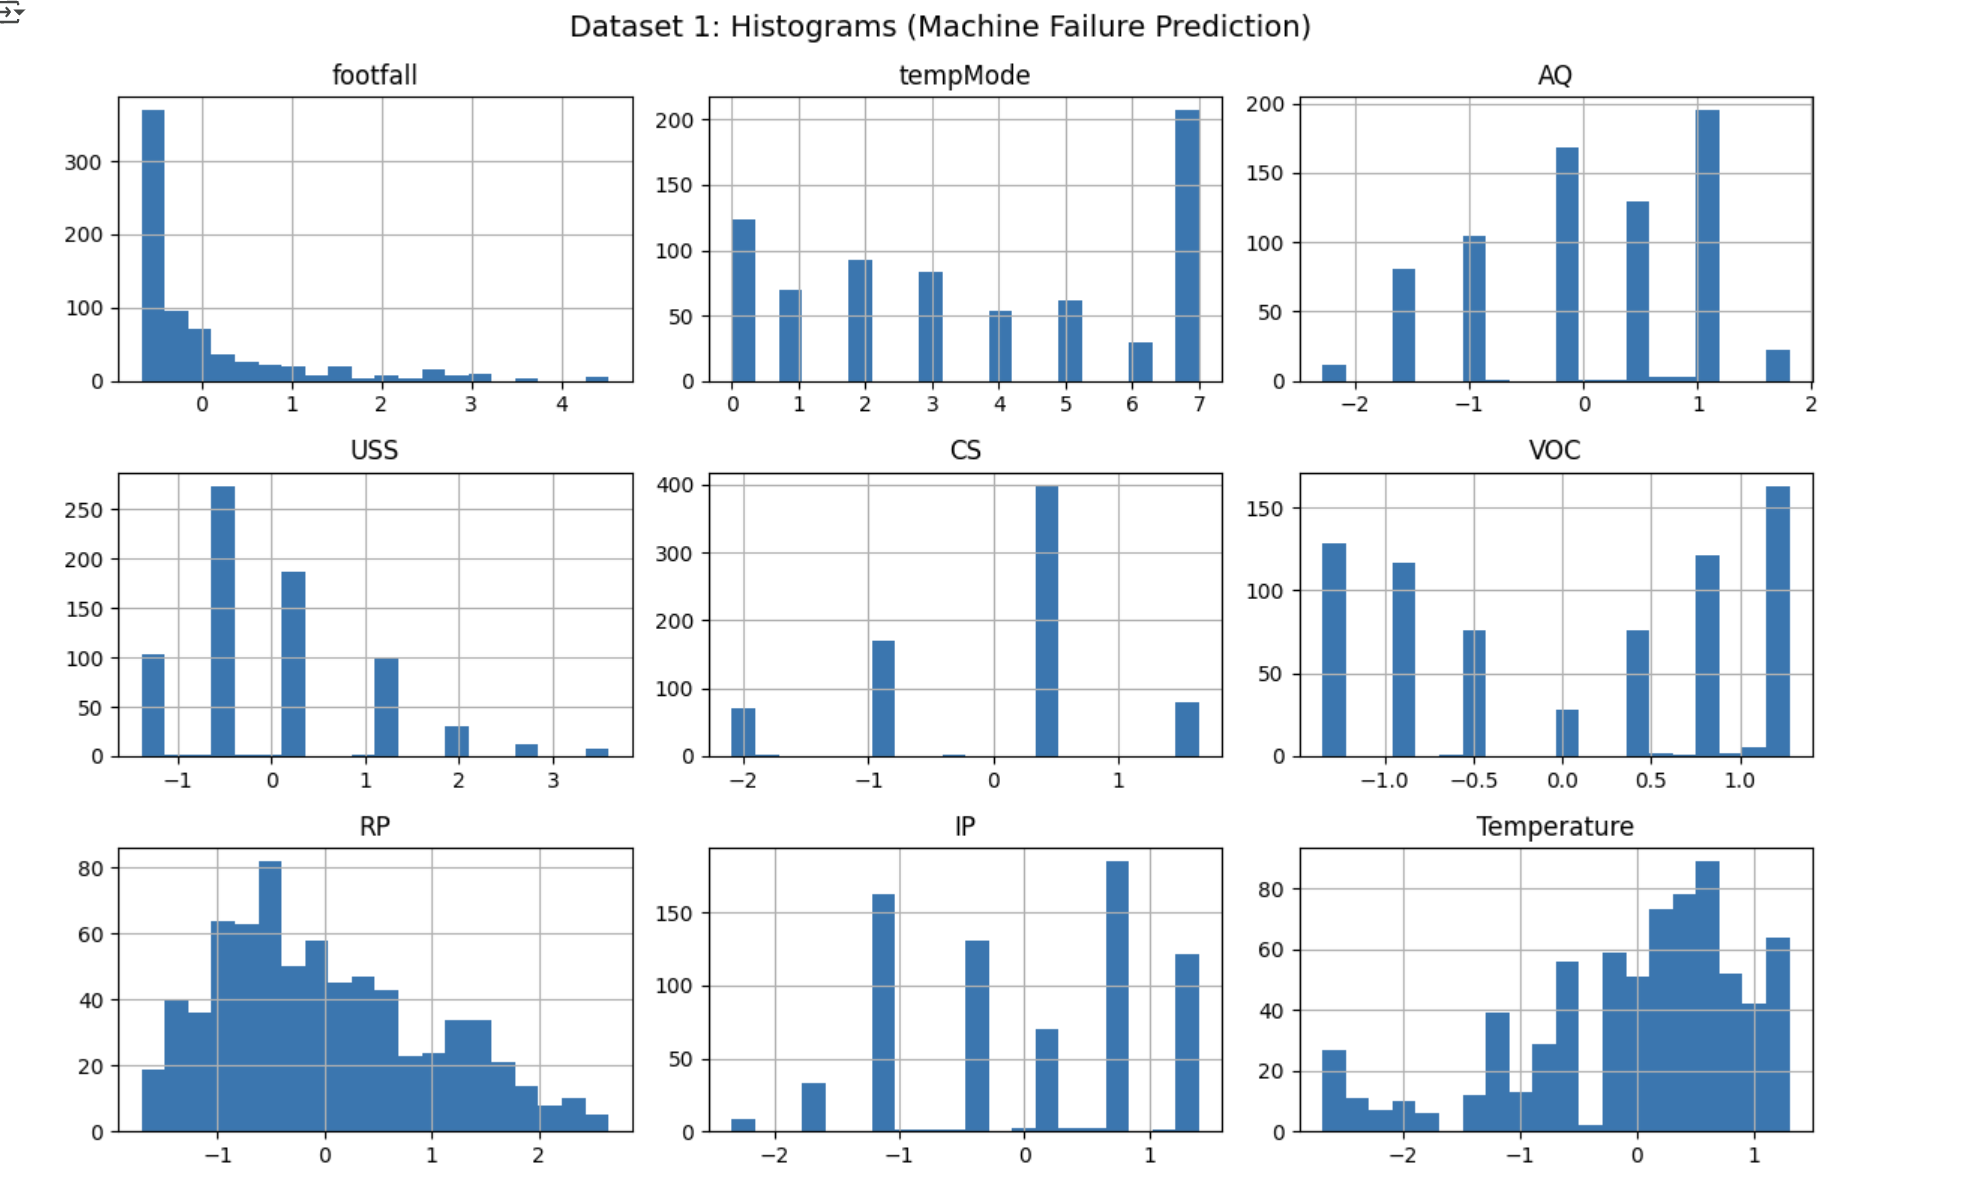
\includegraphics[width=0.8\textwidth]{figures/dataset 1/dataset1_hist.png}
    \caption{Histograms for Dataset 1}
    \label{fig:histograms_dataset1}
\end{figure}

\begin{figure}[h!]
    \centering
    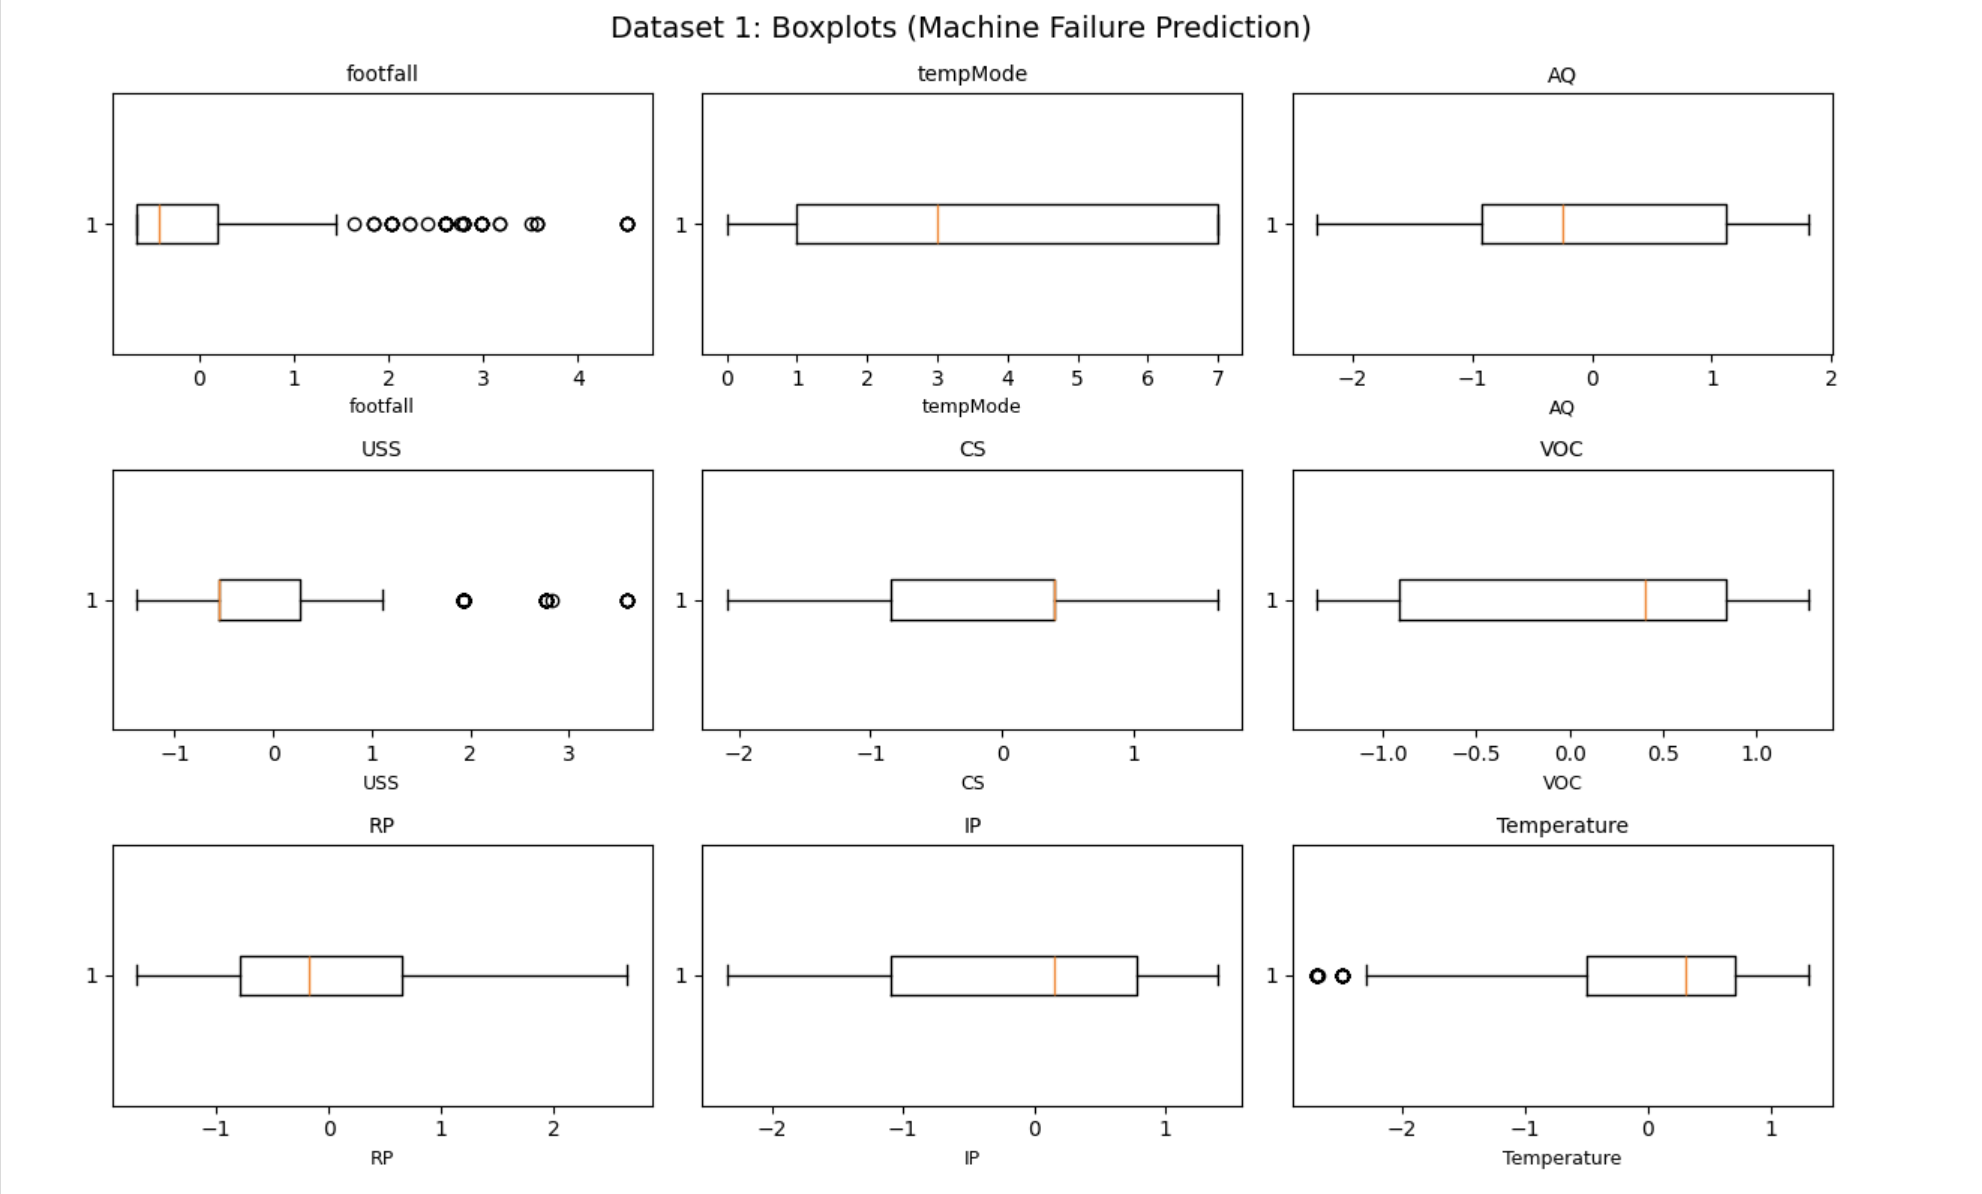
\includegraphics[width=0.8\textwidth]{figures/dataset 1/dataset1_box.png}
    \caption{Boxplots for Dataset 2}
    \label{fig:boxplot_dataset1}
\end{figure}

\begin{figure}[h!]
    \centering
    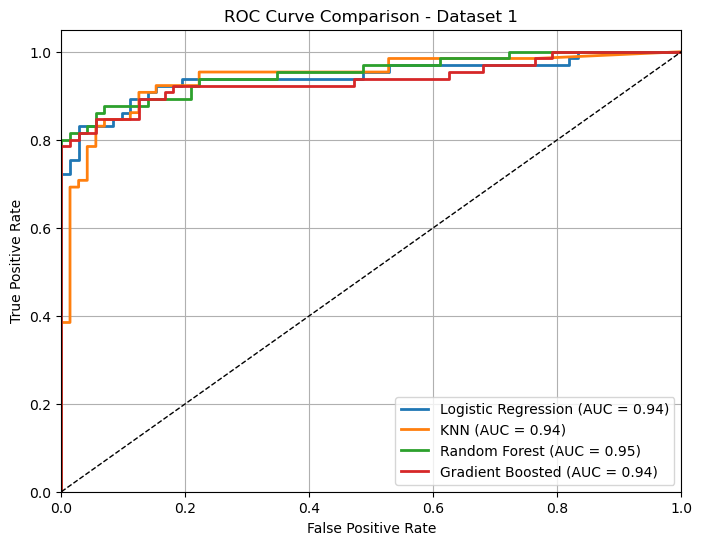
\includegraphics[width=0.8\textwidth]{figures/dataset 1/dataset1_all_models.png}
    \caption{Model Comparison for Dataset 1}
    \label{fig:all_models_dataset1}
\end{figure}

\begin{figure}[h!]
    \centering
    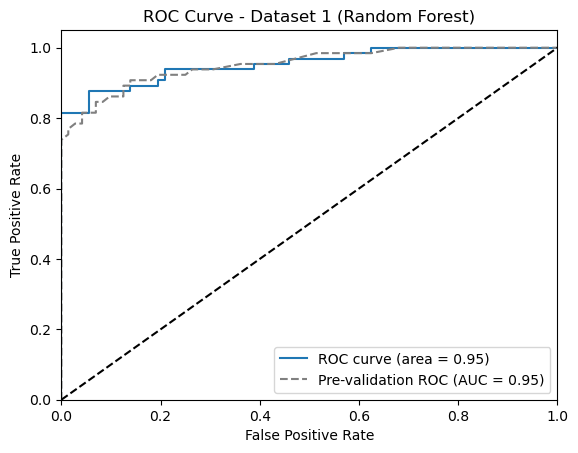
\includegraphics[width=0.8\textwidth]{figures/dataset 1/Dataset1-ROC_curve.png}
    \caption{ROC Curve Comparison for Dataset 1}
    \label{fig:roc_dataset1}
\end{figure}

\begin{figure}[h!]
    \centering
    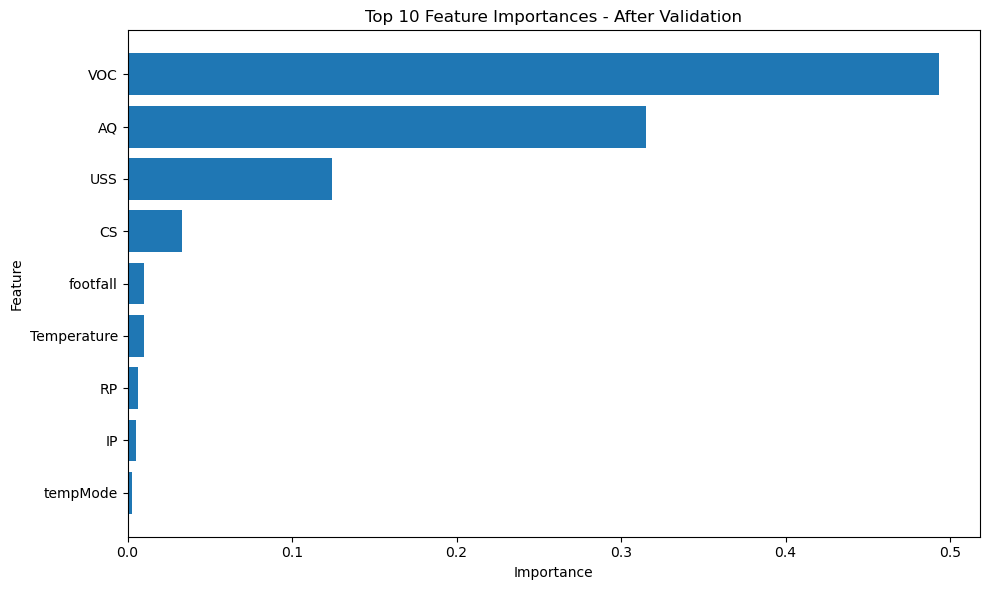
\includegraphics[width=0.8\textwidth]{figures/dataset 1/dataset1_feature_importance.png}
    \caption{Feature importance for Dataset 1}
    \label{fig:feature_importance_dataset1}
\end{figure}

\begin{figure}[h!]
    \centering
    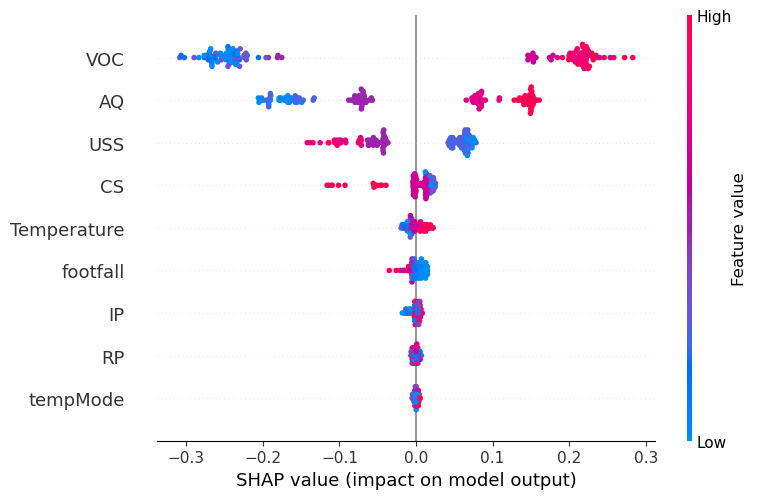
\includegraphics[width=0.8\textwidth]{figures/dataset 1/dataset1_shap_analysis.png}
    \caption{SHAP analysis for Dataset 1}
    \label{fig:shap_analysis_dataset1}
\end{figure}

\begin{figure}[h!]
    \centering
    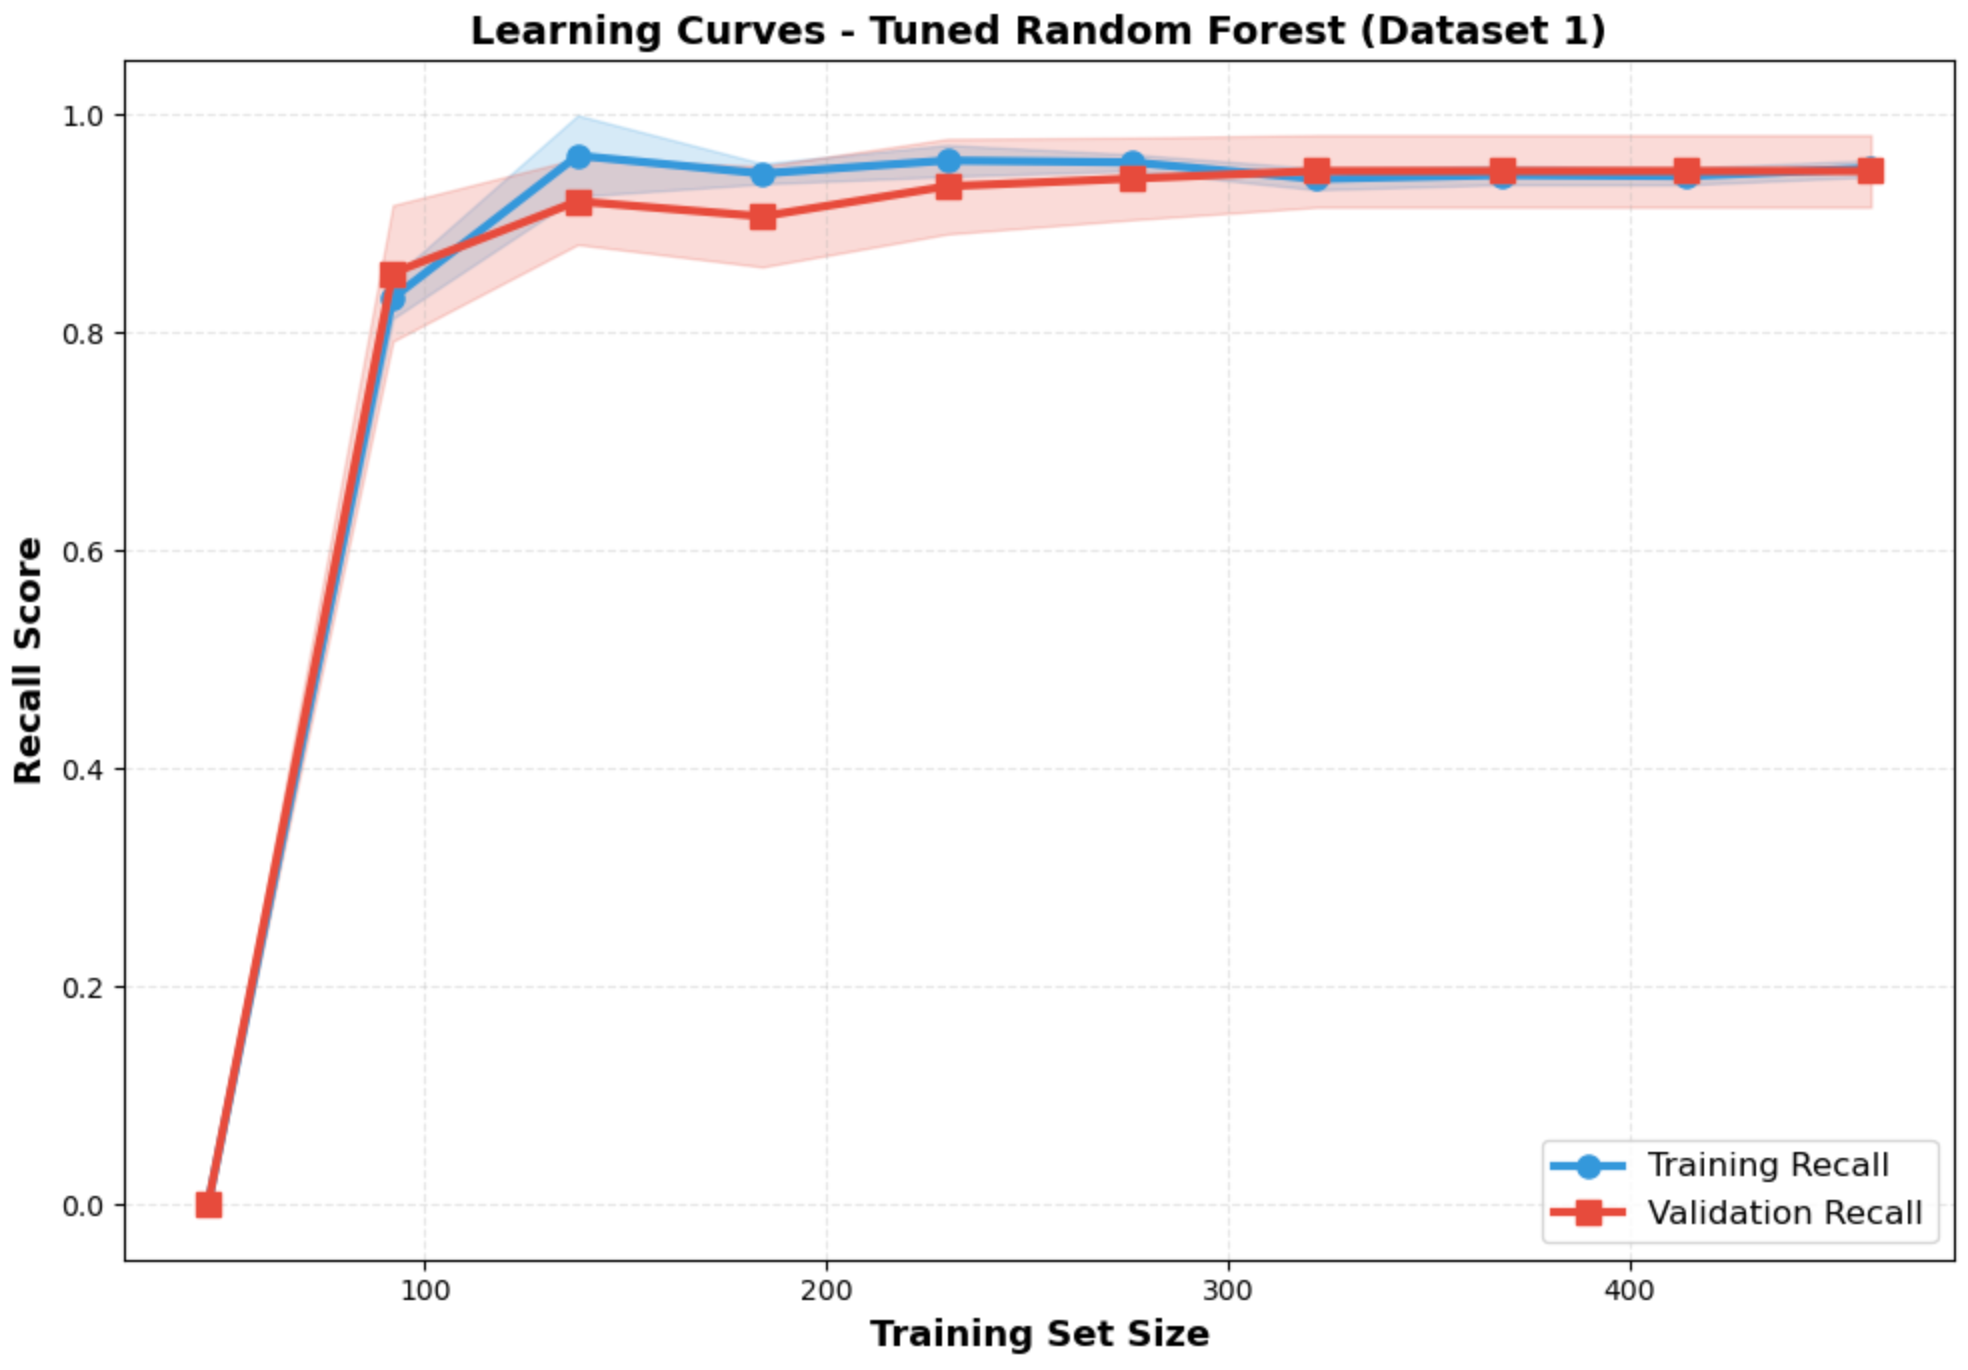
\includegraphics[width=0.8\textwidth]{figures/dataset 1/Dataset1-Learning_Curve.png}
    \caption{Learning Curve Comparison for Dataset 1}
    \label{fig:learning_curve_dataset1}
\end{figure}


%%%%%%%%%%%%%%%%%%%%%%%%%%%%%%%%%%%%%%%%%%%%%%%%%%%%%%%%
%%%%%%%%%%%%%%%%%%%%%%%%%DATASET 2%%%%%%%%%%%%%%%%%%%%%%

\begin{figure}[h!]
    \centering
    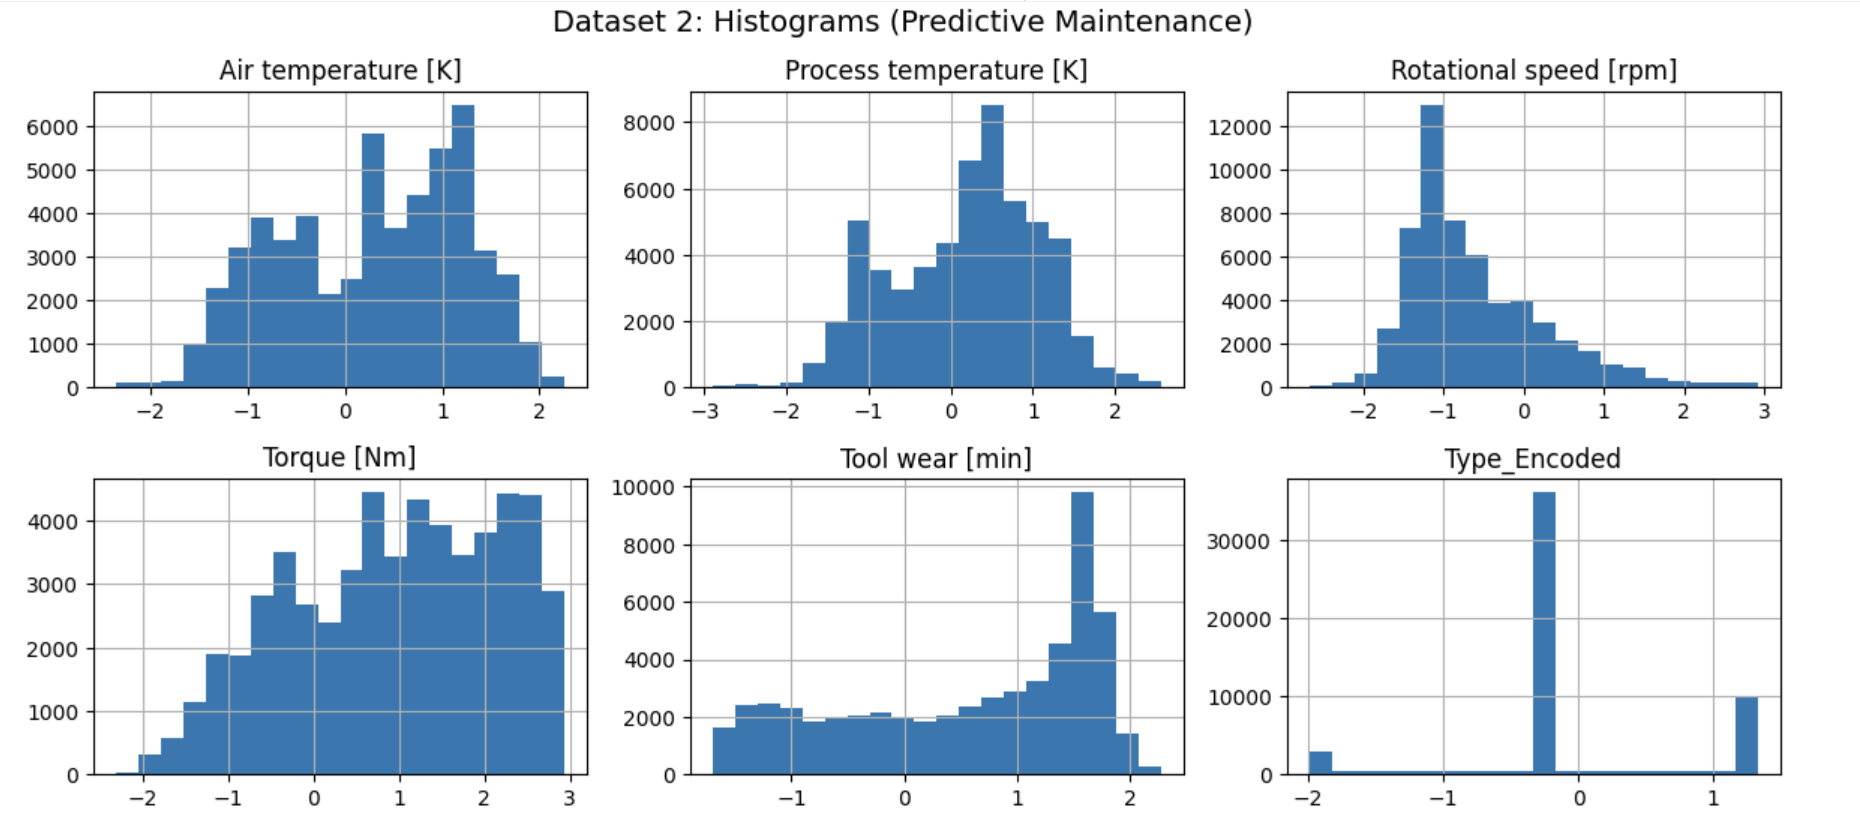
\includegraphics[width=0.8\textwidth]{figures/dataset 2/dataset2_hist.png}
    \caption{Histograms for Dataset 2}
    \label{fig:histograms_dataset2}
\end{figure}

\begin{figure}[h!]
    \centering
    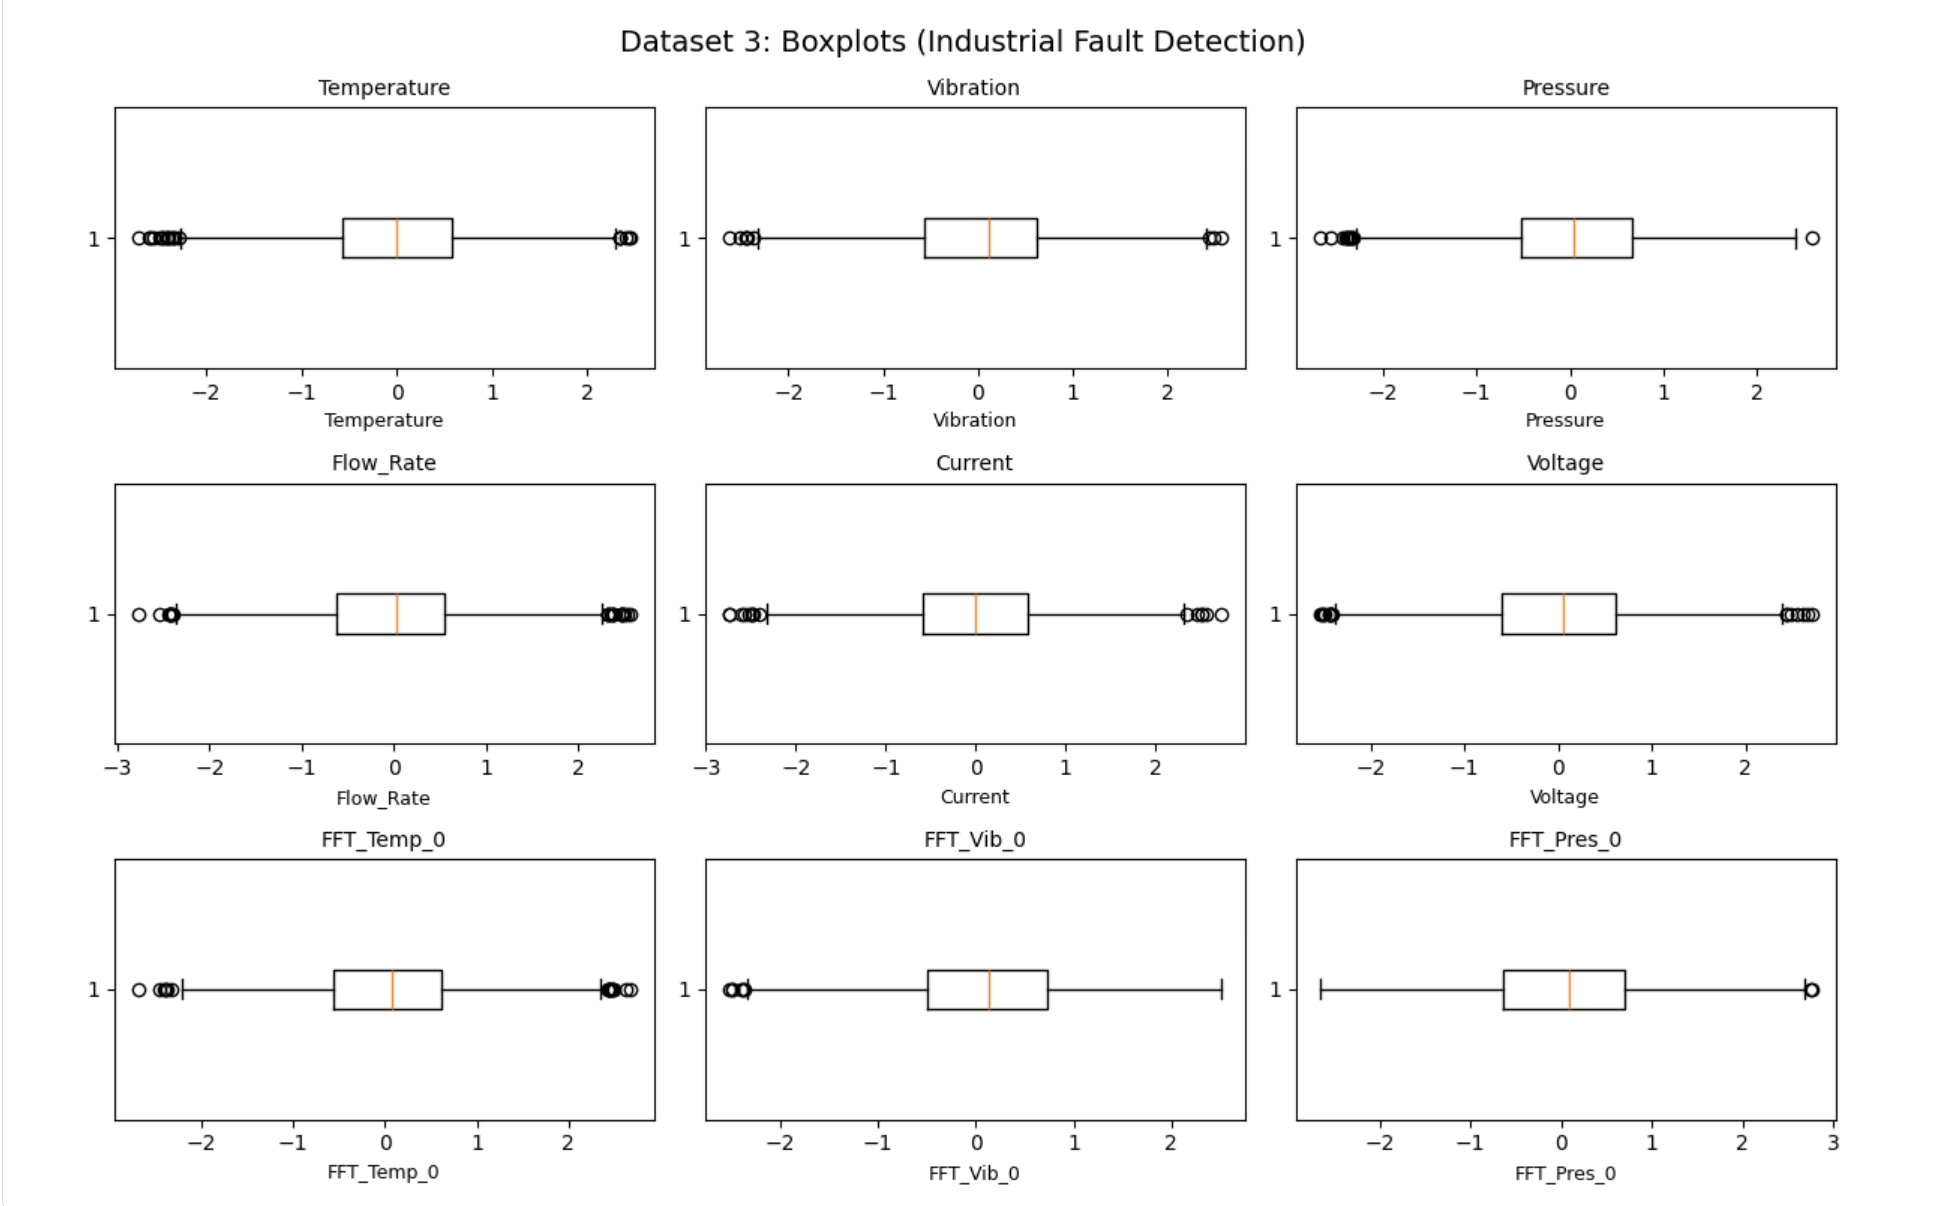
\includegraphics[width=0.8\textwidth]{figures/dataset 3/dataset3_box.png}
    \caption{Boxplots for Dataset 2}
    \label{fig:boxplot_dataset2}
\end{figure}

\begin{figure}[h!]
    \centering
    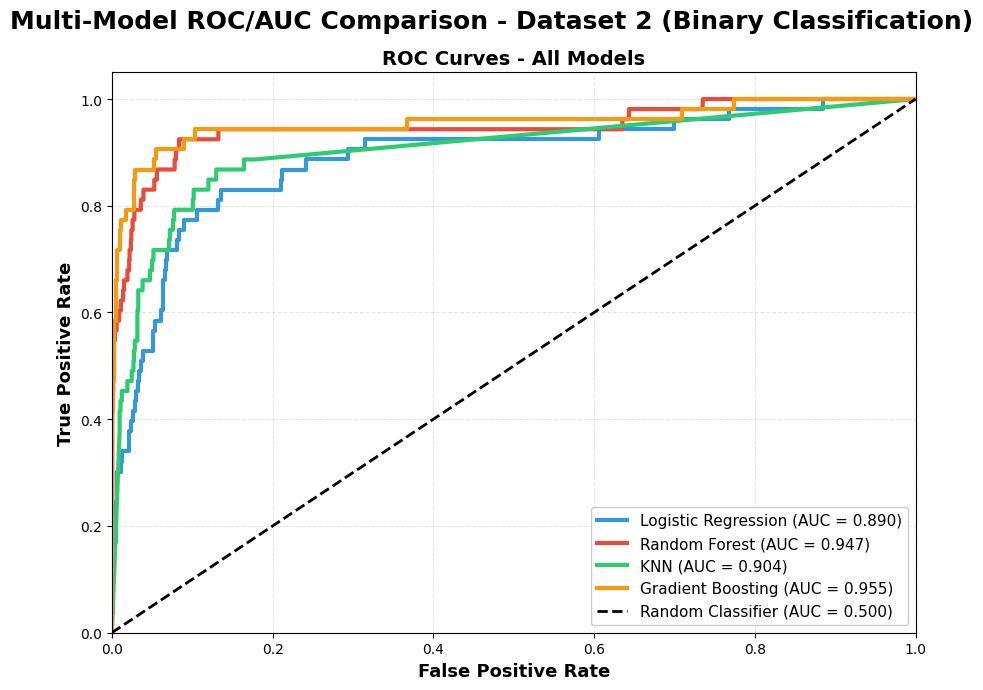
\includegraphics[width=0.8\textwidth]{figures/dataset 2/Dataset 2 multi-model comparison.png}
    \caption{Model Comparison for Dataset 2}
    \label{fig:all_models_dataset2}
\end{figure}

\begin{figure}[h!]
    \centering
    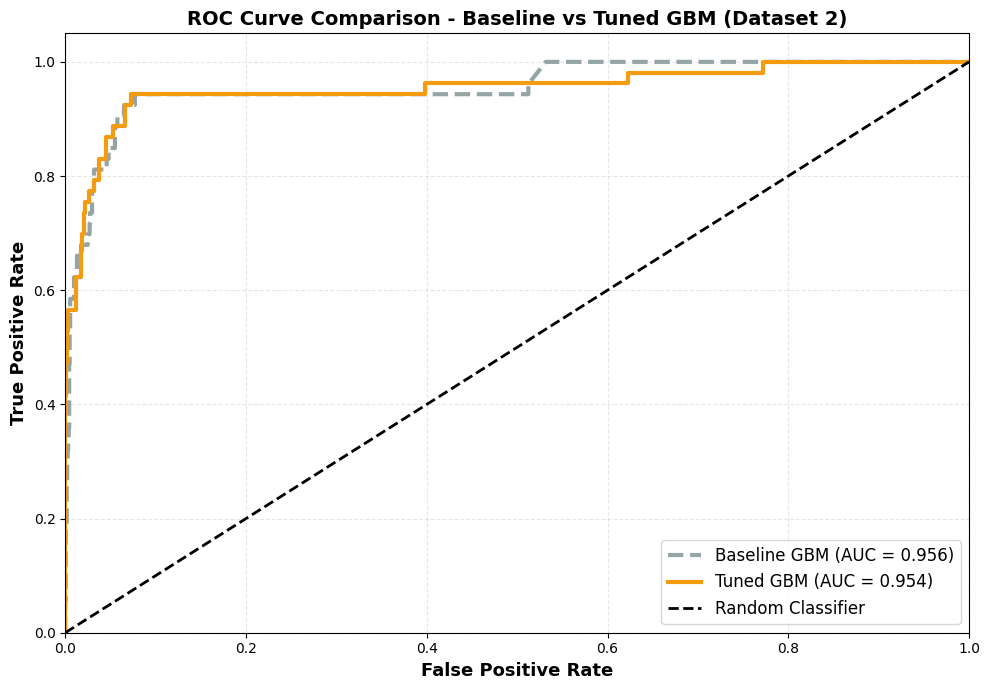
\includegraphics[width=0.8\textwidth]{figures/dataset 2/Dataset 2 baseline vs tuned.png}
    \caption{Baseline vs Tuned Model Comparison for Dataset 2}
    \label{fig:baseline_vs_tuned_dataset2}
\end{figure}

\begin{figure}[h!]
    \centering
    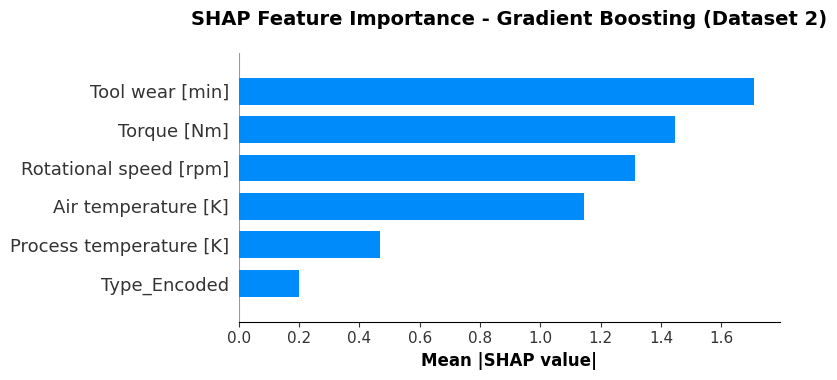
\includegraphics[width=0.8\textwidth]{figures/dataset 2/dataset 2 feature importance bar chart.png}
    \caption{Feature importance for Dataset 2}
    \label{fig:feature_importance_dataset2}
\end{figure}

\begin{figure}[h!]
    \centering
    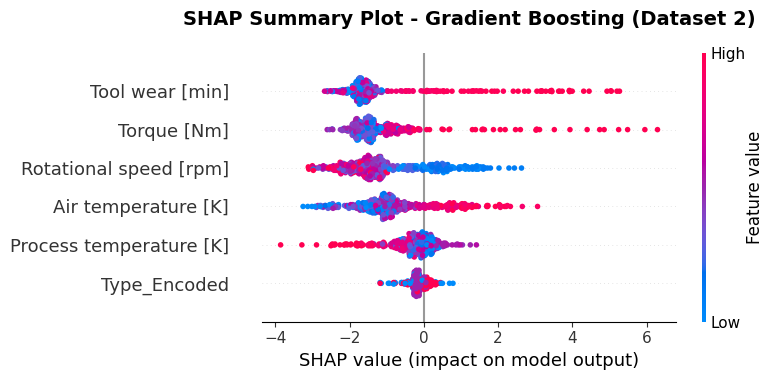
\includegraphics[width=0.8\textwidth]{figures/dataset 2/dataset 2 shap analysis.png}
    \caption{SHAP analysis for Dataset 2}
    \label{fig:shap_analysis_dataset2}
\end{figure}

\begin{figure}[h!]
    \centering
    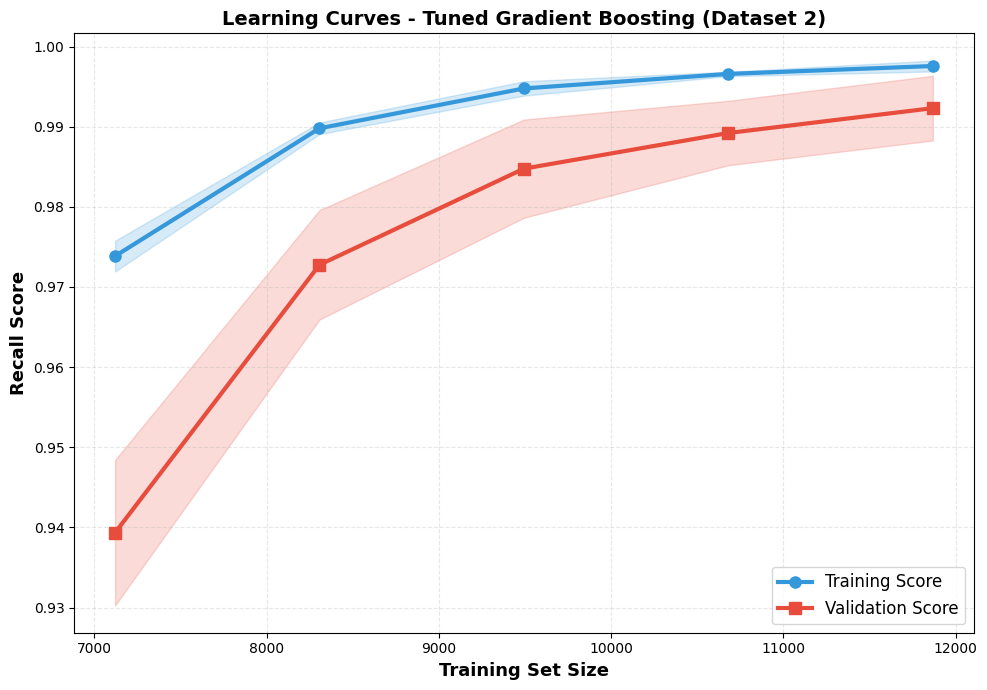
\includegraphics[width=0.8\textwidth]{figures/dataset 2/dataset 2 learning curve.png}
    \caption{Learning Curve Comparison for Dataset 2}
    \label{fig:learning_curve_dataset2}
\end{figure}



%%%%%%%%%%%%%%%%%%%%%%%%%%%%%%%%%%%%%%%%%%%%%%%%%%%%%%%%
%%%%%%%%%%%%%%%%%%%%%%%%%DATASET 3%%%%%%%%%%%%%%%%%%%%%%

\begin{figure}[h!]
    \centering
    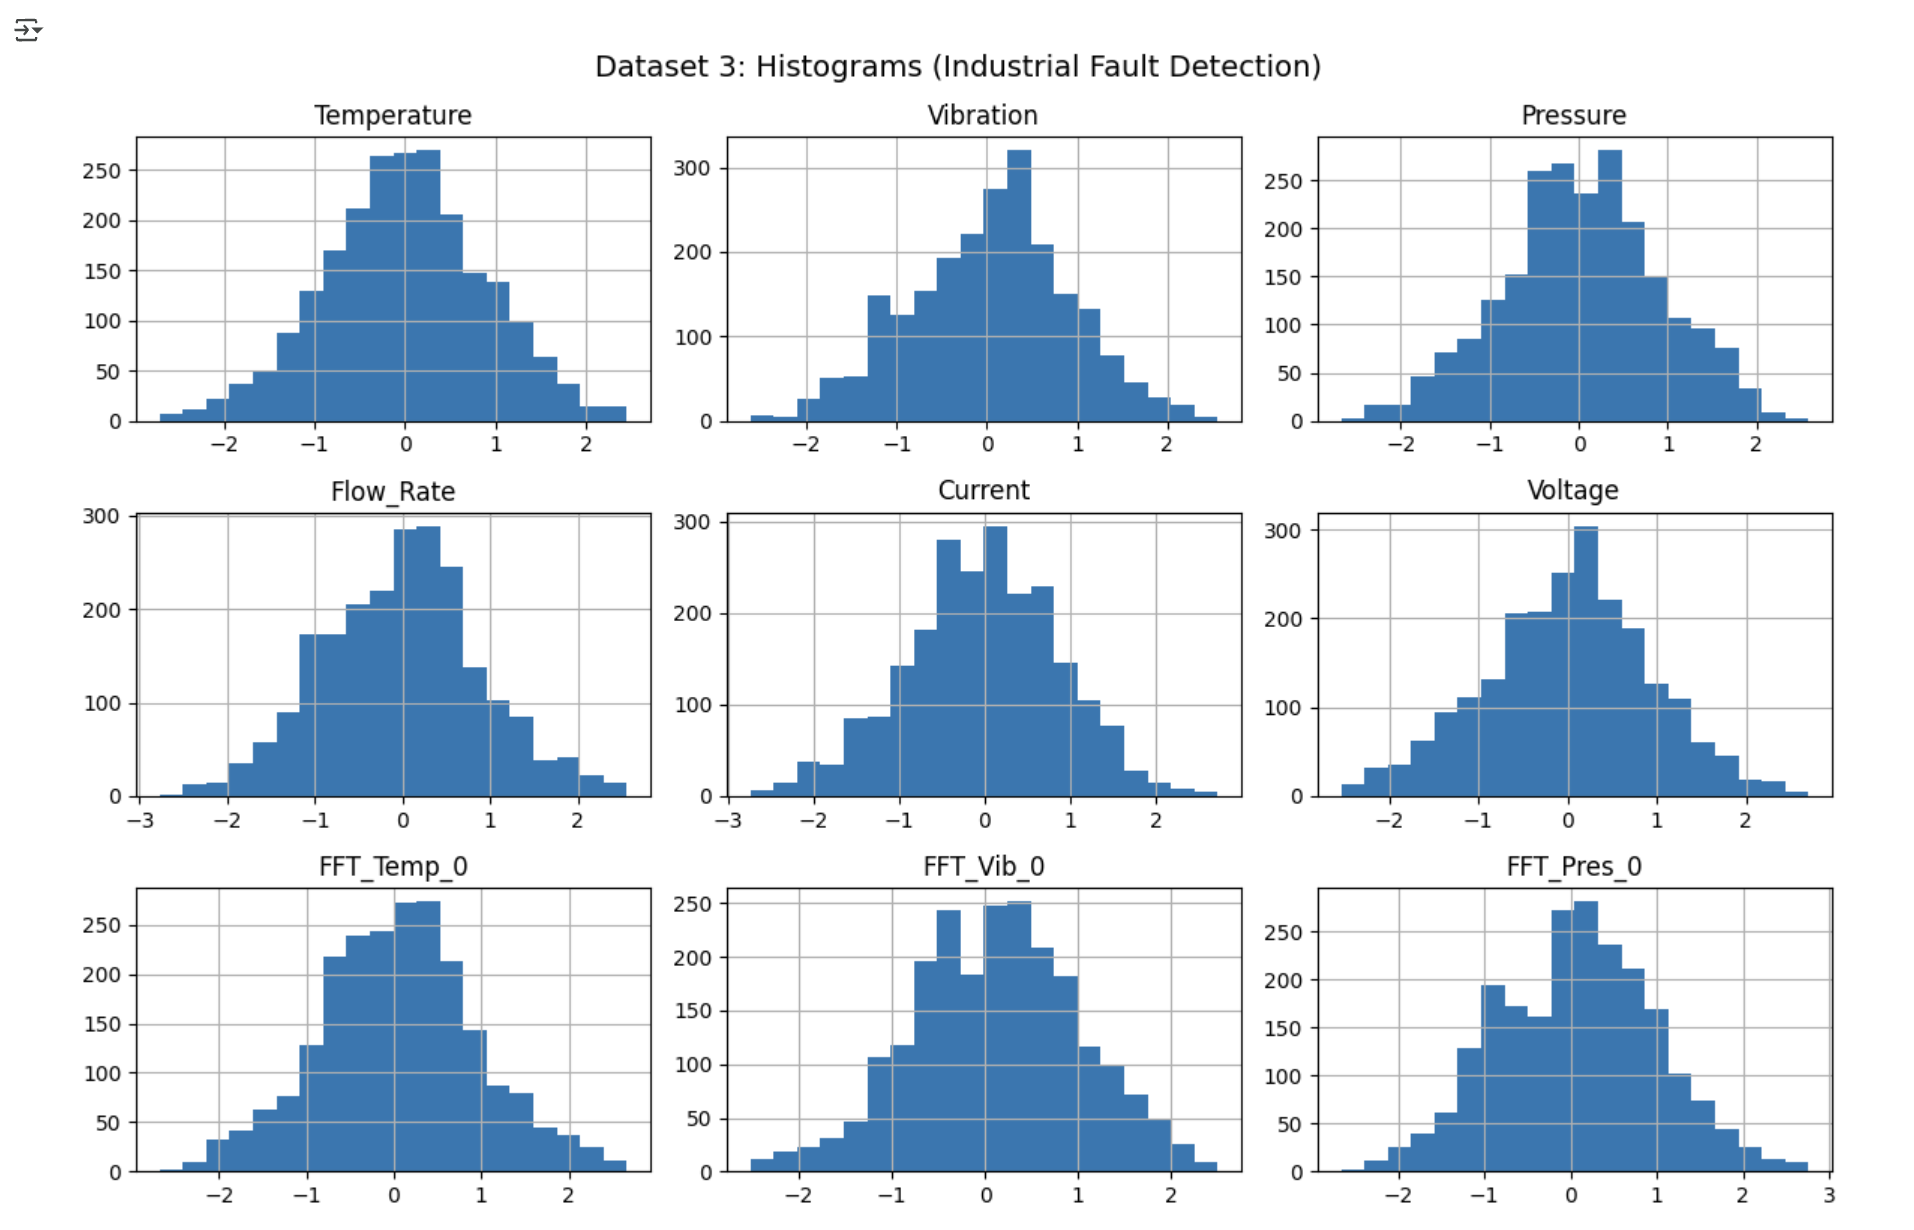
\includegraphics[width=0.8\textwidth]{figures/dataset 3/dataset3_hist.png}
    \caption{Histograms for Dataset 3}
    \label{fig:histograms_dataset3}
\end{figure}

\begin{figure}[h!]
    \centering
    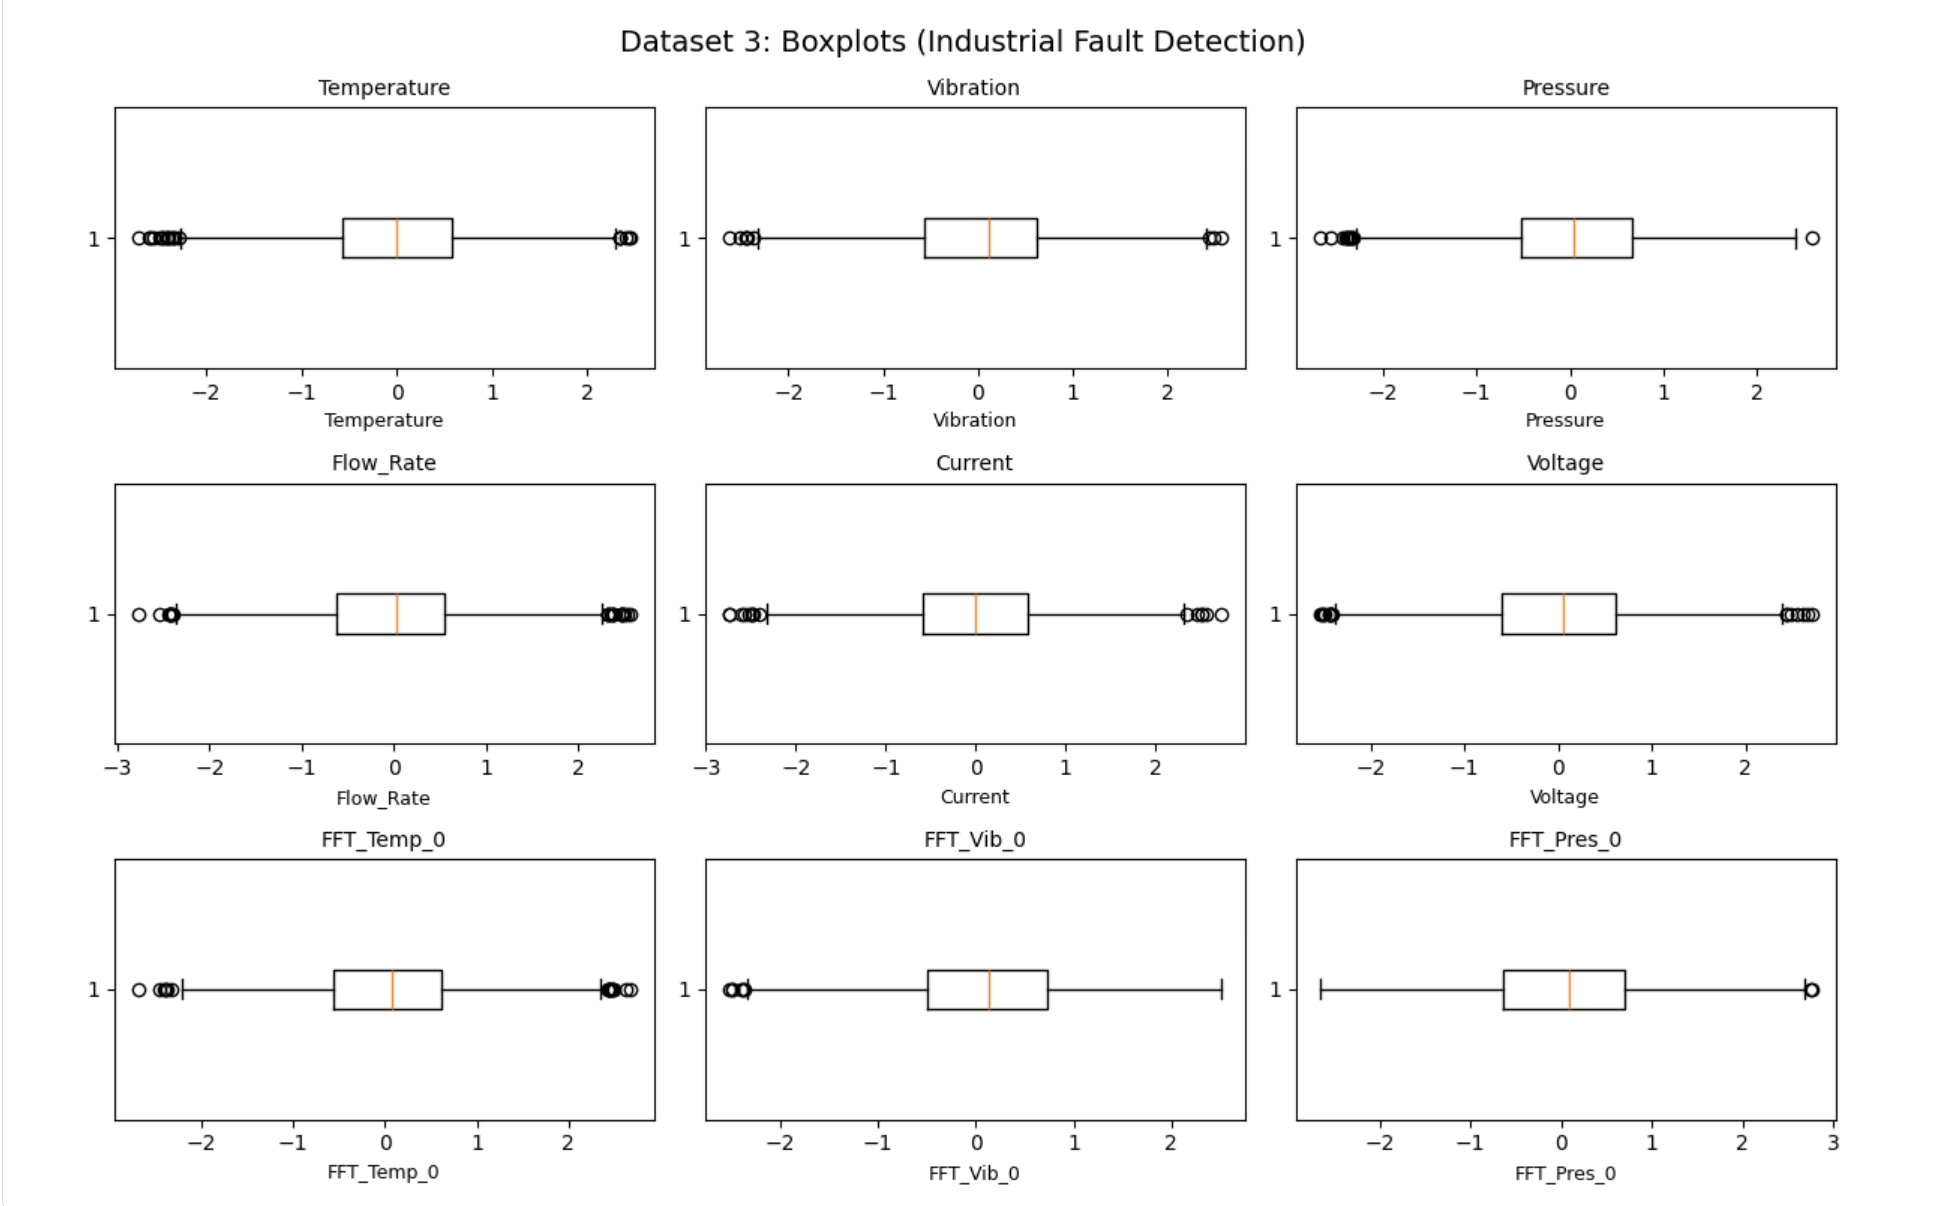
\includegraphics[width=0.8\textwidth]{figures/dataset 3/dataset3_box.png}
    \caption{Boxplots for Dataset 3}
    \label{fig:boxplot_dataset3}
\end{figure}

\begin{figure}[h!]
    \centering
    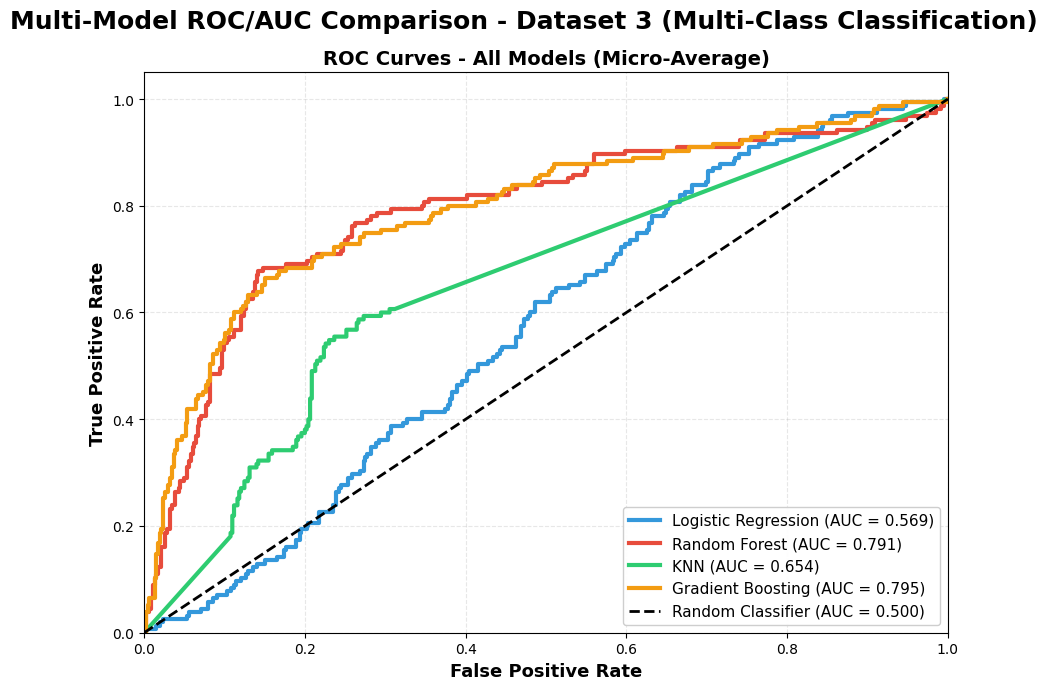
\includegraphics[width=0.8\textwidth]{figures/dataset 3/Dataset 3 multi-model comparison.png}
    \caption{Model Comparison for Dataset 3}
    \label{fig:all_models_dataset3}
\end{figure}

\begin{figure}[h!]
    \centering
    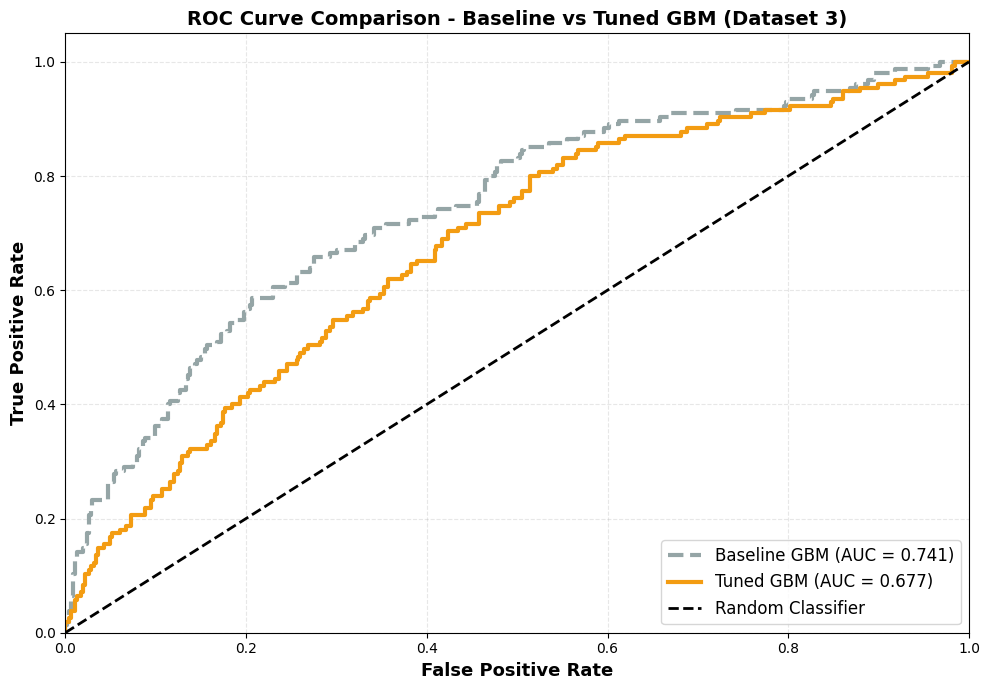
\includegraphics[width=0.8\textwidth]{figures/dataset 3/dataset 3 baseline vs tuned.png}
    \caption{Baseline vs Tuned Model Comparison for Dataset 3}
    \label{fig:baseline_vs_tuned_dataset3}
\end{figure}

\begin{figure}[h!]
    \centering
    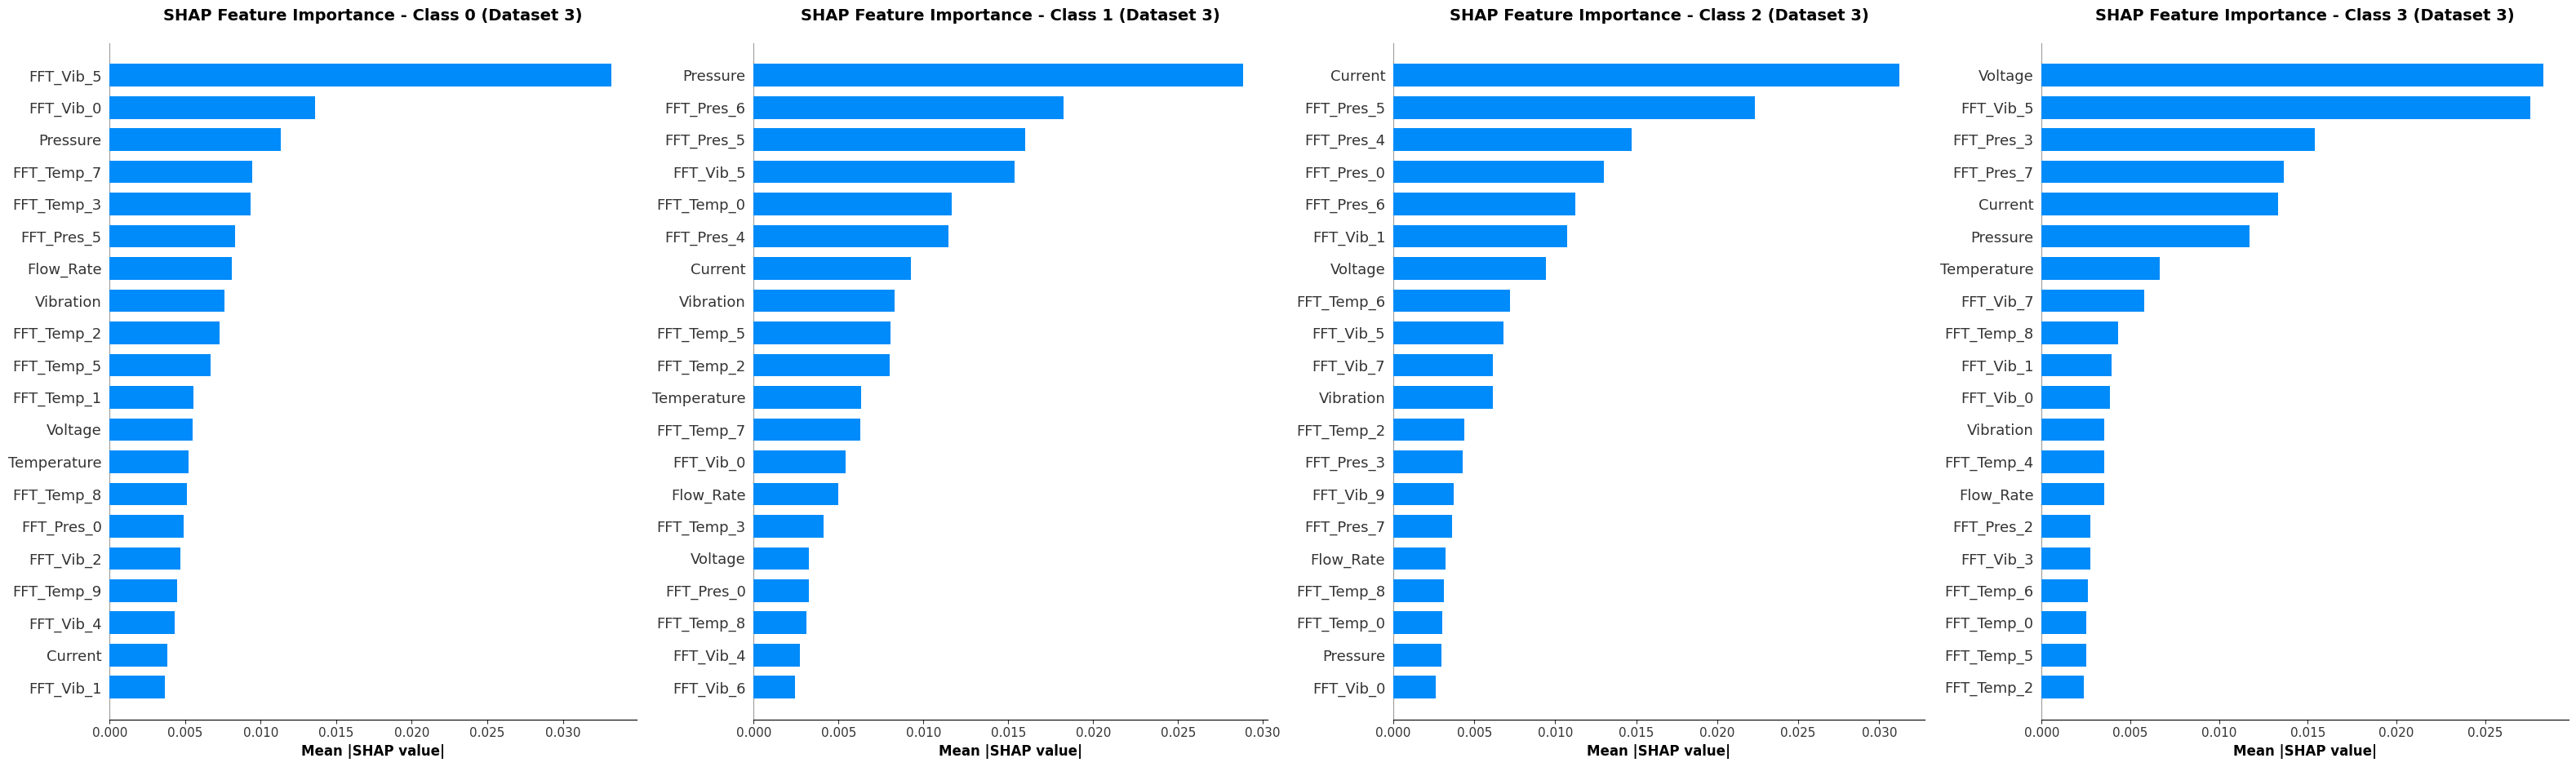
\includegraphics[width=0.8\textwidth]{figures/dataset 3/dataset 3 feature importance merged.jpg}
    \caption{Feature importance for Dataset 3}
    \label{fig:feature_importance_dataset3}
\end{figure}

\begin{figure}[h!]
    \centering
    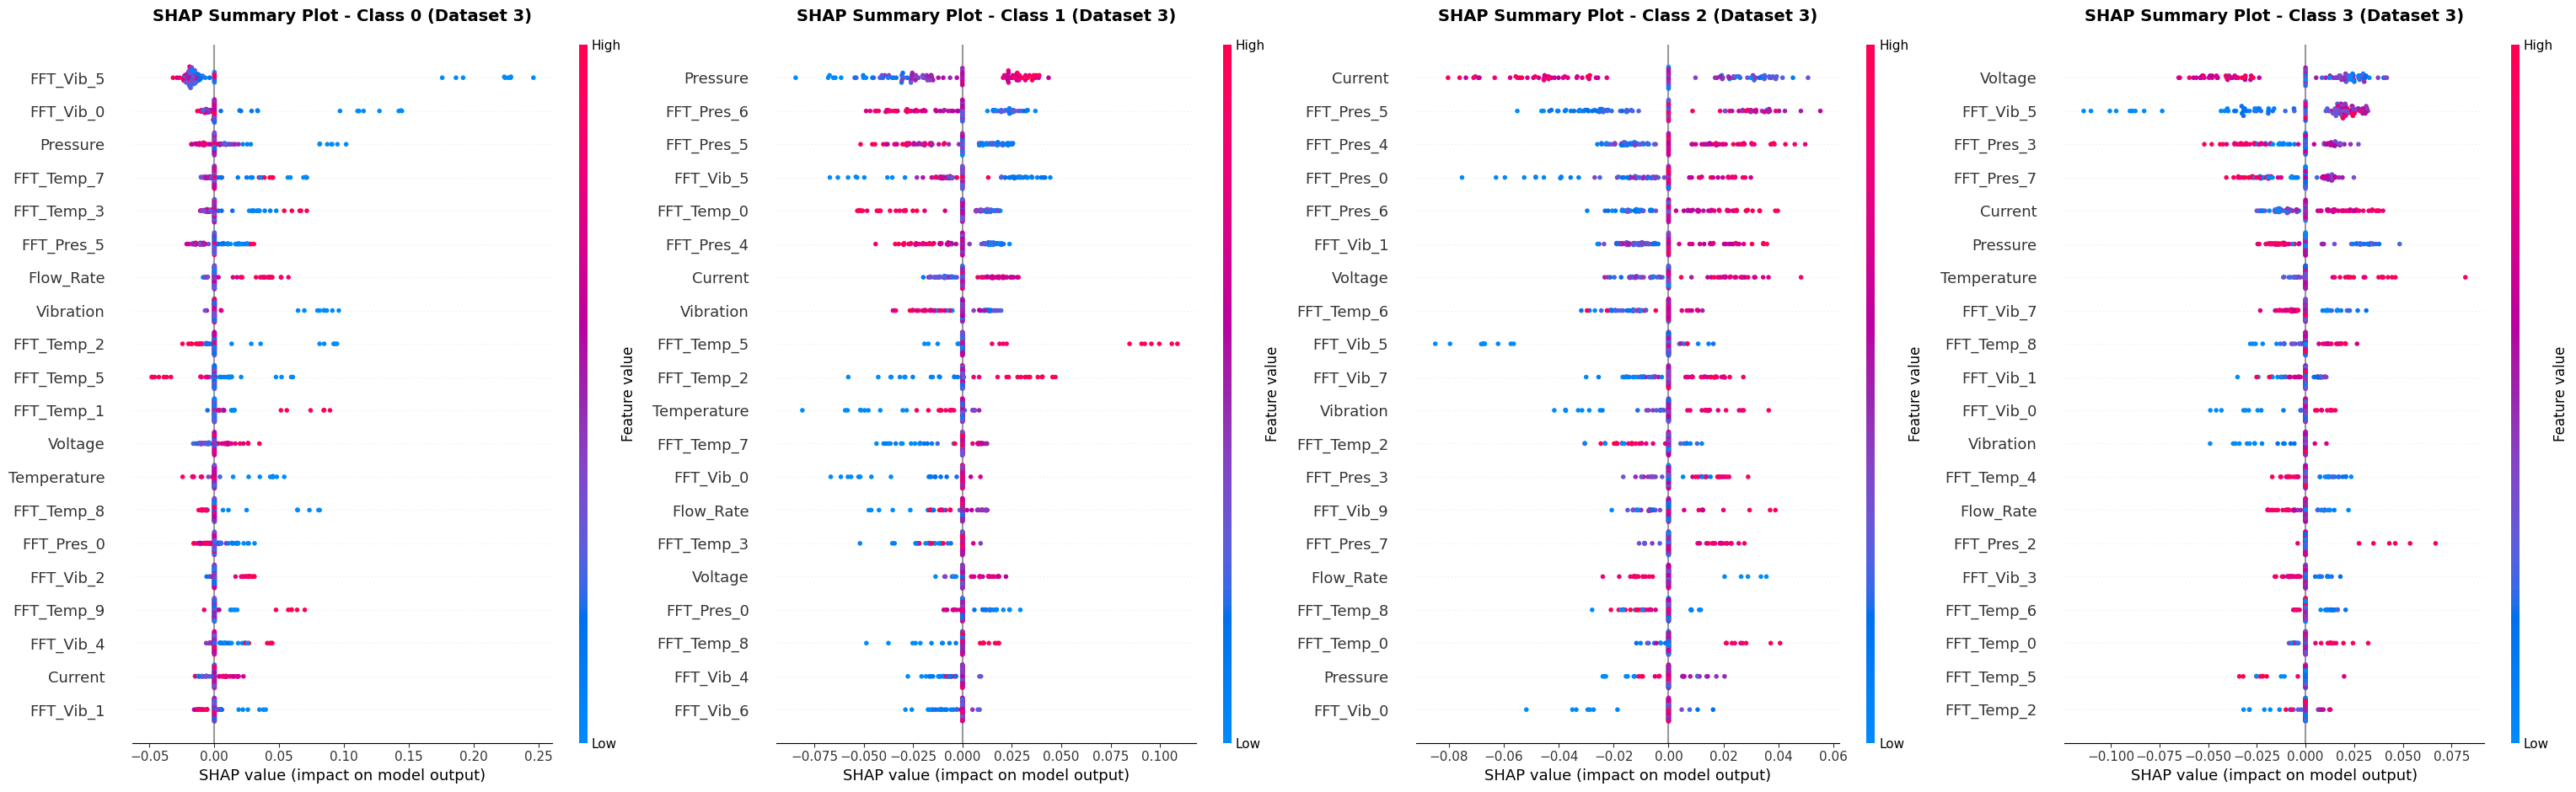
\includegraphics[width=0.8\textwidth]{figures/dataset 3/dataset 3 shap diagram merged.jpg}
    \caption{SHAP analysis for Dataset 3}
    \label{fig:shap_analysis_dataset3}
\end{figure}

\begin{figure}[h!]
    \centering
    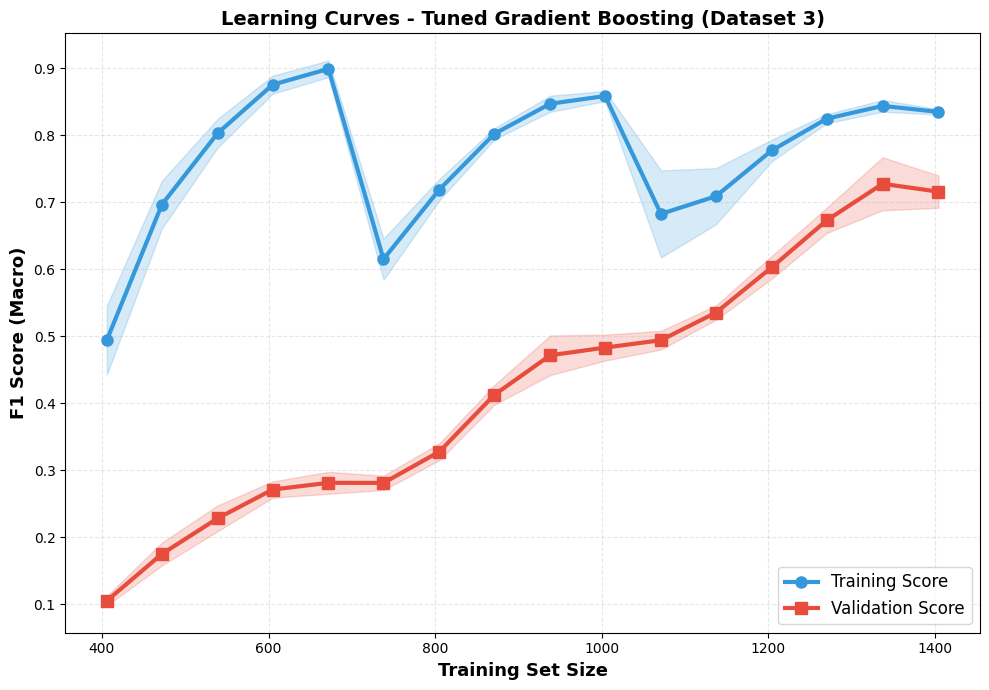
\includegraphics[width=0.8\textwidth]{figures/dataset 3/dataset 3 learning curve.png}
    \caption{Learning Curve Comparison for Dataset 3}
    \label{fig:learning_curve_dataset3}
\end{figure}




\newpage

\end{document}